
%--------------------------------------------------------------------------
% THESIS: The MAIN thesis file from which all other things are included.
%--------------------------------------------------------------------------

% Include the header which includes packages, the Acadia style and definitions.

%---------------------------------------------------------
% Header: This file includes all the packages and custom definitions
% we have used in this example thesis.
%----------------------------------------------------------

% Uncomment the following line if, for some reason, you want a PDF 1.4
% document, rather than (at time of writing) PDF 1.5.
% \pdfminorversion=4

\documentclass[12pt,twoside,openright]{report}

% With these lines, when one tried to copy/paste from AR it does The
% Right Things for ligatures.
\input{glyphtounicode}
\pdfgentounicode=1

%---------------------
% START: Packages
%---------------------
\usepackage{textcomp}
\usepackage[latin1]{inputenc}
\usepackage{amsmath}
\usepackage{amsfonts}
\usepackage{amssymb}
\usepackage{amsthm}
\usepackage{graphicx}
\usepackage{soul}
\usepackage{listings}
\usepackage{subfig}
\usepackage{verbatim}
\usepackage{alltt}
\usepackage{url}

% There are used in the graphics chapter.
% You can delete the following two lines if you use no tikz/pgf graphics
% in your thesis.
\usepackage{tikz}
\usepackage{pgfplots}

% Load the natbib citation package: set the citations to be numerical
% with square brackets separated by commas.
\usepackage[numbers,square,comma]{natbib}

% Now include the Acadia thesis style
\usepackage{acadia-masters-thesis}

% Load the hyperref package.
% The options tell it to (a) use hyper-links to pages with Roman
% numerals that are different than pages with Arabic numbers, and
% (b) tell Adobe reader to show a page number matching the thesis page
% number (rather than sequentially numbering the PDF pages from 1).
\usepackage[plainpages=false,pdfpagelabels]{hyperref}

% The information in the first three lines here goes into the PDF
% document properties.
% The rest of the lines define options related to hyper-links.
% colorlinks: typeset links in the given colours
%	      (otherwise an ugly box is drawn around the links, although
%	       it is only seen on the screen, not in printed copies)
% A newer option (since May 2011) would be to just use the hidelinks option.
% Note: pdfprintscaling=None should discourage Adobe reader from wanting to
% scale your pages to fit printable area when you print from Adobe reader.
\hypersetup{%
    pdftitle={Escaping Local Minima using Symbols},
    pdfauthor={Ahmed Galila},
    pdfkeywords={PUT ANY KEYWORDS HERE},
    colorlinks = true,
    linkcolor = black,
    anchorcolor = black,
    citecolor = black,
    filecolor = black,
    urlcolor = black,
    pdfprintscaling=None
}


% Load the algorithm/mic packages and use chapter-wise numbering
\usepackage{algorithmic}


% JD addition:
% The url package does not, by default, allow breaks at '-'.  Change this
% by adding \do\- to this macro.  If you don't want breaks at '-' in URLs,
% just comment out or delete these lines:
\def\UrlBreaks{\do\.\do\@\do\\\do\/\do\!\do\_\do\|\do\;\do\>\do\]\do\-%
               \do\)\do\,\do\?\do\'\do+\do\=\do\#}%


%---------------------
% END: Packages
%---------------------
%\bibliographystyle{alpha}     % Make citations look like [Smi91], not [12]
\bibliographystyle{plainnat}   % Default boring and almost useless number.

% The depth of the table of contents: change the MAXIMUM depth of
% citations in your table of contents.
\setcounter{tocdepth}{6}

%
% Some definitions of commands used in this thesis
%

% For instance, if you have an acronym you like to use, then define a
% command, it's faster and if the acronym changes you only have to
% change it in one place.
\def\sysacro{SPECIALACRONYM}

% Allow us to change the margins easily and at will
\newenvironment{changemargin}[2]{%
  \begin{list}{}{%
    \setlength{\topsep}{0pt}%
    \setlength{\leftmargin}{#1}%
    \setlength{\rightmargin}{#2}%
    \setlength{\listparindent}{\parindent}%
    \setlength{\itemindent}{\parindent}%
    \setlength{\parsep}{\parskip}%
  }%
  \item[]}{\end{list}}

%setup the default format of listings
\lstset{
    basicstyle=\footnotesize,
    numbers=left,
    xleftmargin=5mm,
    linewidth=\textwidth,
    breaklines,
    frame=tb,
    frameround=fttt
}

% A new definition style
\newtheoremstyle{defstyle}	% name
    {3pt}			% Space above
    {3pt}			% Space below
    {}				% Body font
    {}				% Indent amount
    {\itshape}			% Theorem head font
    {:}				% Punctuation after theorem head
    {.5em}			% Space after theorem head
    {}		% Theorem head spec (can be left empty,meaning 'normal�)
\theoremstyle{definition}
\newtheorem{definition}{Definition}[chapter]


% Change comment style for algorithms
\renewcommand{\algorithmiccomment}[1]{/*#1*/}
% Change Require: to Input: for algorithms
\renewcommand{\algorithmicrequire}{\textbf{Input:}}
% Change Ensure: to Output: for algorithms
\renewcommand{\algorithmicensure}{\textbf{Output:}}

\usepackage[export]{adjustbox}
\graphicspath{ {./imgs/} }

\DeclareMathOperator*{\argmax}{argmax}

\begin{document}

    % PRELIMINARIES: This is the file you will use to setup your
    % name, date, advisor, etc. 
    %---------------------------------------------------------
% Preliminaries: Set up your own details in this file!
%----------------------------------------------------------

\title{Learning with Symbols}
\author{Ahmed Galila}
\dept{Computer Science}
\deptOrSchool{Computer Science}
\degree{Science}

\convocationAndYear{Fall Graduation 2019}
\defenseDate{June 17, 2019}
\copyrightYear{2019}

% Use a "~" after the "r." of "Dr." so that TeX doesn't think you have
% ended a sentence (at which point it gives extra space).
\chair{Dr.~Rob Raeside}
\externalReader{Dr.~Thomas Trappenberg}
\internalReader{Dr.~Greg Lee}
\supervisor{Dr.~Daniel L.~Silver}

% Remove the '%' from the next line and fill in the name if desired.
%\cosupervisor{(Dr.~Your Other Supervisor)}

\headOrDirector{Dr.~Darcy Benoit}
% If the head or director is an ``acting'' head or director, uncomment
% the next line (i.e., delete the '%'):
% \justActing

%-------------------------------------------------------------------------

% This outputs the title page, the approval page and the copyright page.
\firstThreePages

%-------------------------------------------------------------------------

% This outputs the table of contents, lists of figures, tables, ...

\tocAndSuch

%-------------------------------------------------------------------------

\prefacesection{Abstract}
 
The effectiveness of deep neural network models depends on the size and quality of the datasets used to develop these models. Often a lack of sufficient training examples results in the learning algorithm settling into a suboptimal local minima. Individual human learners encounter similar difficulties while learning. However, these challenges are overcome through social interaction and the sharing of learned knowledge in the form of symbols. This thesis presents a hypothesis that states that the presence of clear and concise symbols while training artificial neural networks improves the accuracy of these models when trained on impoverished datasets, similar to how knowledge sharing among humans allows them to overcome their learning difficulties. Empirical studies compare the accuracy of recurrent neural networks, based on long short-term memory units, trained in the presence of symbols with similar networks trained without the benefit of symbols. The models are trained to perform basic arithmetic operations on images of handwritten digits from the MNIST dataset. We try two forms of digit symbol encodings (one-hot and temperature) and compare how well each encoding is able to guide the training process to discover a representation of an algorithm that can generalize to all instances of the problem. The results show that the models trained with the aid of symbols are more effective at performing arithmetic than the models trained without symbols. Furthermore, we show that the temperature encoding of digit symbols are able to capture the quantity and ordinal relationship between the operands and are more effective at discovering an algorithm for each arithmetic operation.

% If you have a list of definitions of abbreviations and symbols used,
% they can go in here.  You will have to do some hand-coding here, but
% if you un-comment the next few lines they will give you an idea,
% depending on how you want to format things.

{\let\cleardoublepage\clearpage\chapter*{Glossary of Terms}}

\begin{itemize}
	\item Adam Optimizer --- A variation of the gradient descent algorithm that maintains a separate learning rate for each network weight.
	\item Auto-encoder --- A type of unsupervised neural network that can learn a compressed encoding of the input features.
	\item Backpropagation Algorithm --- An algorithm that uses gradient descent and the chain rule to determine the weight updates for training multi-layer neural networks.
	\item Backpropagation Through Time (BPTT) --- A variation of the backpropagation algorithm used to train recurrent neural networks.
	\item Bias --- Refers to how much a model deviates from the target function due to incorrect assumptions made about the model.
	\item Constant Error Carousel --- Refers to the recurrent connection in an LSTM unit that allows LSTM networks to learn arbitrary long sequences.
	\item Contrastive Divergence (CD) --- The algorithm used to train RBMs.
	\item Cost Function --- A function used by the gradient descent algorithm to determine how much error a model produces.
	\item Feature Representation --- The way inputs to a neural network are encoded or represented. 
	\item Graphics Processing Unit (GPU) --- A type of processor with an architecture designed specifically for graphics rendering. They are heavily utilized in machine learning due to their highly parallel computing power.
	\item Global Minimum --- The smallest value of a function over its entire domain. 
	\item Gradient Descent Algorithm (GD) --- An algorithm used to calculate the weight updates of a neural network based on the error produced when applying the training data to the network.
	\item Internal Feature --- The output from the hidden layer nodes of a neural network that is fed into the next layer.
	\item Internal Representation --- The weights of the internal connections of a neural network.
	\item Least Significant Digit --- The lowest digit of a number located on the far right of a string representing the number.
	\item Local Minimum --- The smallest value of a function over a specific range.
	\item Long Short-Term Memory (LSTM) --- A type of neural network unit used to replace perceptrons in recurrent neural networks (RNNs) that allows RNNs to remember and model long sequences of data.
	\item MNIST Dataset --- A dataset composed of images of handwritten digits often used by machine learning and computer vision researchers to train handwritten digit classifiers.
	\item Most Significant Digit --- The highest digit of a number located on the far left of a string representing the number.
	\item One-Hot Vector --- A type of feature encoding that represents a digit as a vector where all the elements are set to zero except for the element corresponding to the digit being represented which is set to one.
	\item Ordinal Relationship --- A relationship between numbers that determines whether a number comes before or after another number. 
	\item Recurrent Neural Network (RNN) --- A type of artificial neural networks that can model temporal data.
	\item Restricted Boltzman Machine (RBM) --- A type of auto-encoder based on Boltzman Machines where cyclic connections are not allowed.
	\item Symbol --- A clear, concise and consistent representation of noisy input data. A symbol of a specific concept will have one and only one representation.
	\item Stochastic Gradient Descent --- A variation of the gradient descent algorithm that updates the weights after every training example is introduced instead of waiting for all training examples to be processed in an epoch.  
	\item Temperature Encoding --- A type of feature encoding that represents a digit as a vector that has as many values sequentially set to one, starting from the right, as the integer being represented.
	\item Variance --- Determines how much a model is affected by the training data.
\end{itemize}

%-------------------------------------------------------------------------
% Now write your acknowledgements (if any).
% If you wish to acknowledge no-one, delete or comment-out the
% next few lines.

%\Acknowledgments

%Place any acknowledgments you might want to make here.

%\noindent
%Don't forget to be formal and professional.

%-------------------------------------------------------------------------

% Don't mess with this line!
\afterpreface


    % CHAPTER CONTENT START
    % Replace all the lines from here down to ``CHAPTER CONTENT END''
    % with a collection of ``\include{XYZ}'' lines, where each such XYZ
    % is the name of a text file holding (for example) one chapter of
    % your thesis.
    % If you have appendices you need that ``\appendix'' line BEFORE
    % you \include your appendices.
    \chapter{Introduction} \label{sec:introduction}

Imagine you are lost in a jungle, wandering alone in an unfamiliar environment fraught with danger and uncertainty. Your survival depends on your ability to learn to differentiate between the things you can eat and the things that can eat you. This is an expensive and risky process given the need for movement and trial and error. One day you come across another individual that is more familiar with your surroundings. Together you develop a common sign language (symbols) that you can use to know more about the threats and opportunities in this hostile environment. Along with real examples, these symbols allow you to overcome your struggle in the jungle.

Learning in humans involves being introduced to many examples. The more examples the learner is exposed to the more effective the learning process is. This however is not always possible given the cost (energy and time) and risk (injury and death) involved. The ability of a single learner to learn effectively is therefore hampered by the lack of a sufficient number of examples. However, societies evolved to overcome this challenge by developing mechanisms by which accumulated knowledge is shared amongst individuals in the group\cite{DBLP:journals/corr/abs-1203-2990}.

Similar to how the lack of a sufficient number of examples can make learning difficult for humans, machine learning models also experience difficulty in finding a suitable representation when they are trained with a limited dataset. The research presented in this thesis draws analogies between training neural network models and learning in humans.  We investigate how the presence of symbols while training artificial neural networks with impoverished datasets can improve the effectiveness of these models, just like the exchange of symbols between individual human learners can help them overcome their learning challenges.

We begin this chapter by providing a brief introduction to machine learning and specifically deep learning followed by an overview of learning with symbols. We then discuss our research scope and objective. Finally, we present an outline to the remainder of the thesis.

\section{Machine Learning with Neural Networks} \label{sec:introduction-introduction-machine-learning}

Designing computer systems that can model the world in such a way as to exhibit what we call intelligence requires such systems to have the ability to interpret a large number of factors. For example, if we were to develop a system that can identify and perform calculations using numbers from images of handwritten digits, the system would have to account for all the possible variations in which each digit can be written. Given the amount of data required, it would be infeasible to manually formalize solutions to these problems. Machine Learning algorithms can instead be used to automate the development of a solution by learning the important features that represent the problem domain and formalize them in a way that can then be applied to different instances of the problem\cite{Bengio:2009:LDA:1658423.1658424}.

\subsection{Neural Networks} \label{sec:introduction-introduction-machine-learning-neural-networks}

Many advances in artificial intelligence (AI) research are inspired by work done in other fields, specifically those that aim to study human cognition, language and social interaction\cite{DBLP:journals/corr/abs-1203-2990}. Deep learning, which is a form of machine learning, is one particular area of AI that is heavily influenced by how the human brain works.

In deep learning, models are constructed to represent tasks (problems) using processing units called artificial neurons that are inspired by how biological neurons function in living organisms. These neurons are connected in layers to form artificial neural networks, that when properly trained, have the power to represent solutions to these complex problems. Section \ref{sec:background-artificial-neural-networks} provides a detailed description of artificial neural networks.

When training neural network models, an appropriate set of weights is discovered that allows the network to capture the factors of variation exhibited in the problem and therefore approximate an unknown function $f$. The training process requires a set of training examples that are applied iteratively to the model. After each iteration, the error produced by the model is calculated and the model parameters are updated in such a way as to attempt to reduce that error in subsequent iterations. The goal of the learning algorithm is to discover the approximating function $\hat{f}$ that will accurately generalize to yet unseen examples.


\subsection{Challenges in Training Neural Networks} \label{sec:introduction-introduction-machine-learning-challenges-training-neural-networks}

There are two factors that affect the effectiveness (accuracy) of a trained model, namely the variance exhibited in the training examples and the bias assumed in the model. Variance refers to how much the model errs because of changes in the training data, whereas the bias of a model refers to how much the model errs because of incorrect assumptions made by the learning algorithm approximating $\hat{f}$ when compared to the real function $f$. An ideal model will exhibit both low variance and low bias\cite{James:2014:ISL:2517747}.

The variance factor tells us that the size and quality of our training dataset has a huge impact on the quality of the models being developed. The larger the training set and greater the algorithm's representation power, the more accurate our models will be\cite{James:2014:ISL:2517747}. The next section introduces a theory, that including symbols of noisy concepts helps overcome the challenges of training neural networks from small impoverished datasets. Symbols provide concise and accurate information to the learning algorithm that can assist in forming more accurate models.

\section{Learning with Symbols} \label{sec:introduction-learning-symbols}

Humans generally don't need as many training examples to learn a specific concept or task compared to machine learning systems. For example, a human learner can learn to identify an object in an image using only a single example. When we contrast that with an artificial neural network, the neural network might need hundreds of examples to achieve the same level of accuracy. We as humans build on the knowledge we've accumulated over our lifetimes\cite{Thrun1998}. Designing deep learning systems that accumulate and integrate knowledge over time and over multiple tasks is therefore important to overcome the challenge of learning from impoverished datasets\cite{silver2013lifelong}.

When considering how learning in humans works, it is believed that the ability of individual humans to learn new concepts accurately is hampered by the number and variety of examples of the concepts they are each exposed to. However, this difficulty is overcome when individuals communicate concise examples of concepts between each other using a common language\cite{DBLP:journals/corr/abs-1203-2990}. This common language, which we refer to in this thesis as symbols, is very effective at transferring the knowledge, that has accumulated in a society over a long period of time, from one generation to the next.

Deep artificial neural networks experience similar challenges when learning new concepts from limited datasets. This can be attributed to the existence of many local minima in the hypothesis space of the network's loss function\cite{Larochelle:2009:EST:1577069.1577070}. We therefore hypothesize that similar to how human learners use symbols to overcome difficulty in learning from limited real examples, artificial neural networks can also benefit from symbols to improve the effectiveness (accuracy) of training using a limited dataset.

The research presented in this thesis empirically investigates the effect of introducing a clear and consistent symbolic channel on the accuracy of neural network models. We propose that the clear symbols introduced during training introduce inductive bias to the network which guides the training algorithm to a more optimal representation\cite{Thrun1998}. The next section states the objective and scope of our research.

\section{Research Objective and Scope} \label{sec:introduction-research-objective-scope}

Our goal is to draw parallels between our understanding of how humans learn with symbols and how learning with symbols can best be applied to machine learning algorithms. The objective is to demonstrate that providing clear and concise knowledge in the form of symbols to a deep neural network can improve the effectiveness of the training process by significantly reducing the number of noisy training examples needed to produce a high level of accuracy.

\subsection{Research Objective} \label{sec:introduction-research-objective-scope-research-objective}

Knowledge sharing will be empirically demonstrated in this thesis by training deep neural networks to perform basic arithmetic operations (such as addition, subtraction, multiplication and division) on images of handwritten digits. These models will accept the images as inputs and will output the result of the operation as vectors that encode the value of the output. The models will also accept a symbolic channel that emulates shared knowledge between learning agents. Training will be performed with and without the presence of symbols. The results will then be analyzed to show the impact of the symbolic channel on the accuracy of the models developed.

Besides showing that the presence of symbols increases the accuracy of artificial neural networks, we also want to empirically explain why symbols allow for this improvement. In deep neural networks, layers of the architecture learn abstractions that can be shared among different tasks\cite{Bengio:2009:LDA:1658423.1658424}. We believe that some of these abstractions can be learned more effectively from clear symbols than they can from noisy inputs. This leads to better models than if the networks were trained using noisy handwritten digits alone.

\subsection{Scope} \label{sec:introduction-research-objective-scope-scope}

We focus our research on understanding the effect of symbols on the accuracy of deep neural networks, we also examine the effectiveness of different approaches to encode and provide symbols to our neural network models. Several models are developed to investigate the effects of symbols on training accuracy and to a lesser extent on the speed of training. This thesis presents the results obtained from these experiments as well as an analysis of these results. We limit our experiments to developing neural network architectures using recurrent neural networks based on Long Short Term Memory units (LSTMs). The application domain is also limited to training the LSTM networks to learn to perform addition, subtraction, multiplication and division on images of handwritten digits from the MNIST dataset (see Section \ref{sec:theory-approach-the-mnist-dataset}).

Other types of neural network architectures, such as Convolutional Neural Networks, will not be considered for this problem. MNIST images are preprocessed so that all digits are centered and are of the same orientation and scale. It has been shown that traditional feed-forward networks can perform very well on the MNIST dataset without the need for convolution. Therefore, in order to reduce complexity and focus on the problem at hand, convolutional neural networks are not used. 

\section{Thesis Outline} \label{sec:introduction-thesis-outline}

This chapter introduced the basis for our theory and the goal and strategy of our research. The following is an outline of the remaining chapters in this thesis.

Chapter 2 introduces the background knowledge that is required by the reader in order to understand the remainder of the thesis. We start Chapter 2 by introducing artificial neural networks (Section \ref{sec:background-artificial-neural-networks}), including a discussion on deep learning. Next, in Section \ref{sec:background-sequence-modeling}, a detailed explanation of recurrent neural networks (RNNs) and long short-term memory units (LSTMs) is presented. These models form an important aspect of our empirical studies. Finally, Section \ref{sec:background-problem-local-minima} wraps up Chapter 2 by introducing the core problem that our theory is based on, that of local minima.

Chapter 3 formally lays out the hypothesis that forms the basis for our research. This is followed by an explanation of our theory development and the approach being proposed to investigate and validate this theory. 

Chapter 4 presents the empirical studies used to test and further develop the theory. Each experiment performed is detailed along with the results and a discussion of those results.

Chapter 5 is the last chapter and provides a summary of our findings and contributions. We also suggest avenues for future work.
    \chapter{Background} \label{sec:background}

The previous chapter discusses how machine learning algorithms are used to allow computer systems to solve problems that would otherwise be impossible to achieve with traditional programming languages. Artificial neural networks, which are inspired by the neural networks found in living organisms, provide a mechanism to represent solutions to such problems. In this chapter, we take a deeper look at how artificial neural networks are constructed and trained as well as the difficulties and challenges they present.

We begin by describing the artificial neuron (Section \ref{sec:background-artificial-neural-networks-perceptron}), which is the basic building block of artificial neural networks, followed by a description of the gradient descent algorithm, which is used to train these neurons. Then in Section \ref{sec:background-artificial-neural-networks-feed-forward-neural-networks} we explain how we can build more complex models by combining many neurons. In Section \ref{sec:background-deep-learning} we discuss the advantages of deep learning, which involves combining several layers of neurons. Section \ref{sec:background-problem-local-minima} explains the problem of local minima which forms a major challenge to effectively train deep neural networks and which comprises the core of the problem we are solving in this thesis. Finally, in Section \ref{sec:background-sequence-modeling}, we explain recurrent neural networks which are a specialized form of neural networks that allow for modeling of sequential data and which are heavily utilized in the experiments presented in Chapter 4.

\section{Artificial Neural Networks} \label{sec:background-artificial-neural-networks}

The goal of any machine learning system is to learn a function $\hat{f}$ that approximates a target function $f$. In supervised learning, the approximating function might be a classifier of the form $\hat{f}(x) = y$ that learns to map an input vector $\vec{x}$ to a category $\vec{y}$\cite{Goodfellow-et-al-2016}. For example, a system can be made to classify images of handwritten digits into their corresponding values from zero to nine. In this case, when properly learned, the approximate function will accept a vector ($\vec{x}$) that represents the intensities of each pixel in the image and output a vector ($\vec{y}$) representing the class of the image from zero to nine.

There are four components to any machine learning system. First there is the training data from which the learning system acquires the rules that make up the target function, the target function itself, the target function's representation and finally the learning algorithm that updates the representation's parameters to allow the representation to approximate the target function\cite{Mitchell}. Artificial neural networks are one form of target function representation that are inspired by the nervous systems found in living organisms and form the basis of deep learning models.

Artificial neural networks consist of artificial neurons that are mathematical models of a single neuron in a natural nervous system. These artificial neurons accept weighted inputs and produce an output if the sum of the inputs meet a certain threshold. Many neurons can be linked together to form a network. The goal of the learning algorithm is to find a suitable set of weights, which correspond to the synaptic weights found in natural nervous systems, that allow the network to produce the correct output of the function $f(\vec{x})$ given any input $\vec{x}$ in $f$'s domain. That way, the resulting model is said to represent the target function $f$. The remainder of this section provides a detailed look at neural networks and the learning algorithms associated with them.

\subsection{The Perceptron} \label{sec:background-artificial-neural-networks-perceptron}

\begin{figure}[t]
	\centering
	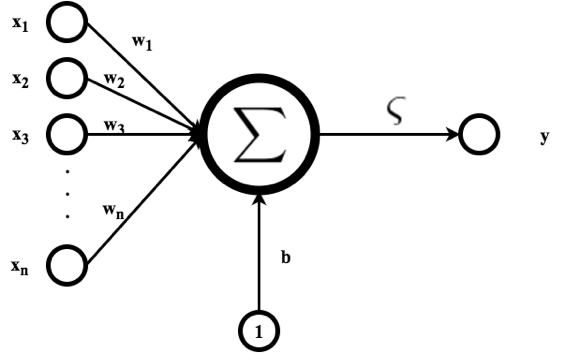
\includegraphics[max width=\textwidth]{perceptron}
	\caption{Visual depiction of a single artificial neuron, sometimes called a perceptron.}
	\label{fig:perceptron}
\end{figure}

Consider the problem of classifying a set of data points into one of several classes. We can reduce this problem to that of finding a decision function $\hat{f}(\vec{x})$ that approximates a true function $f(\vec{x})$, that maps a data point $\vec{x}$ to a class $\vec{y}$. The function $f(\vec{x})$ can be represented as a linear combination of the parameters of $\vec{x}$:
\begin{gather*}
	w_1 x_1 + w_2 x_2 + ... + w_n x_n + b = y_1\\
	w_1 x_1 + w_2 x_2 + ... + w_n x_n + b = y_2\\
	\vdots\\ 
	w_1 x_1 + w_2 x_2 + ... + w_n x_n + b = y_m
\end{gather*}
The problem of learning the decision function then becomes finding a set of weights ($w_1$ to $w_n$ and $b$) that satisfy the provided data points as well as generalize to yet unseen observations\cite{Le15atutorial}.

This system of equations can be depicted as a neuron, like that shown in Figure \ref{fig:perceptron}, that accepts weighted inputs and fires an output that is modified by an activation function. The weights in an artificial neuron resemble synaptic weights found in the neural networks of living organisms. Synaptic weights determine how much influence one neuron has on the next in the network. When considered in the context of artificial neural networks, the weights determine how much the corresponding part of the input affects the output and therefore they act as the medium by which the network is able to represent the decision function\cite{Mitchell}.  

The activation function on the other hand resembles the threshold potential of a natural neural network. It determines how the signal propagates through the system. Likewise, the activation functions of artificial neural networks determine the shape of the output of each unit. Figure \ref{fig:perceptron} shows a neuron with a sigmoid activation. The sigmoid activation function normalizes the output of the unit to a value between zero and one and also produces a non-linear output which is important for some functions\cite{Goodfellow-et-al-2016}.

Once fully trained, the neuron (also called a perceptron) is then used to predict the output of unseen observations using the following formulas:
\begin{gather}
\label{eq:sigmoid}
	z = b + \sum\limits_{i=1}^n x_i w_i\\
	y = \frac{1}{1+e^{-z}}
\end{gather}

\subsubsection{Gradient Descent Algorithm}

The process of discovering the optimum set of weights is performed using the gradient descent algorithm. Gradient descent involves updating the weights of the model in such a way as to minimize the error produced by  applying the training examples to the perceptron relative to the expected target output. The error is depicted as a cost function whose gradient we need to traverse in the negative direction to minimize the error. See Figure \ref{fig:gradient-descent}\cite{Le15atutorial}. The mean square error (MSE) is a popular cost function\cite{Mitchell} given by:
\begin{equation}
E(\vec{w}) = \frac{1}{2} \sum_{d \in D} (t_d - y_d)^2
\end{equation}
where $\vec{w}$ is a vector that comprises the neuron's weights, $D$ is the set of training examples, $t_d$ is the target output for the training example $d$ and $y_d$ is the actual output of the perceptron for training example $d$. 

Figure \ref{fig:gradient-descent} visualizes the error function. Initially the weights are set to random values that place the error at an undesirable level. By iteratively updating the weights, the error is reduced and the weights evolve to capture the decision function. The weight update rule for a linear perceptron where:
\begin{equation}
	y = b + \sum\limits_{i=1}^n x_i w_i\\
\end{equation}
is given by:
\begin{equation}
w_i \leftarrow w_i + \Delta w_i
\end{equation}
where
\begin{equation}
\Delta w_i = -\eta \frac{\partial E}{\partial w_i}
\end{equation}
$\eta$ is the learning rate. The learning rate is a positive value that determines the step size that the gradient descent will take. The larger the learning rate the quicker the descent, however this risks skipping over the optimal weights.

The change $\Delta w_i$ can be obtained by partially differentiating the error with respect to $w_i$:
\begin{equation}
\begin{split}
\frac{\partial E}{\partial w_i} & = \frac{\partial}{\partial w_i} \frac{1}{2} \sum_{d \in D} (t_d - y_d)^2\\
& = \frac{1}{2} \sum_{d \in D} \frac{\partial}{\partial w_i} (t_d - y_d)^2\\
& = \frac{1}{2} \sum_{d \in D} 2(t_d - y_d) \frac{\partial}{\partial w_i} (t_d - y_d) \\
& = \sum_{d \in D} (t_d - y_d) \frac{\partial}{\partial w_i} (t_d - \vec{w}.\vec{x_d}) \\
& = \sum_{d \in D} (t_d - y_d) (-x_{id})
\end{split}
\end{equation}
where $x_{id}$ is the input of training example $d$. The update rule is therefore given by:
\begin{equation} \label{eq:weight-update}
\Delta w_i = \eta \sum_{d \in D} (t_d - y_d) (x_{id})
\end{equation}

\begin{figure}[t]
	\centering
	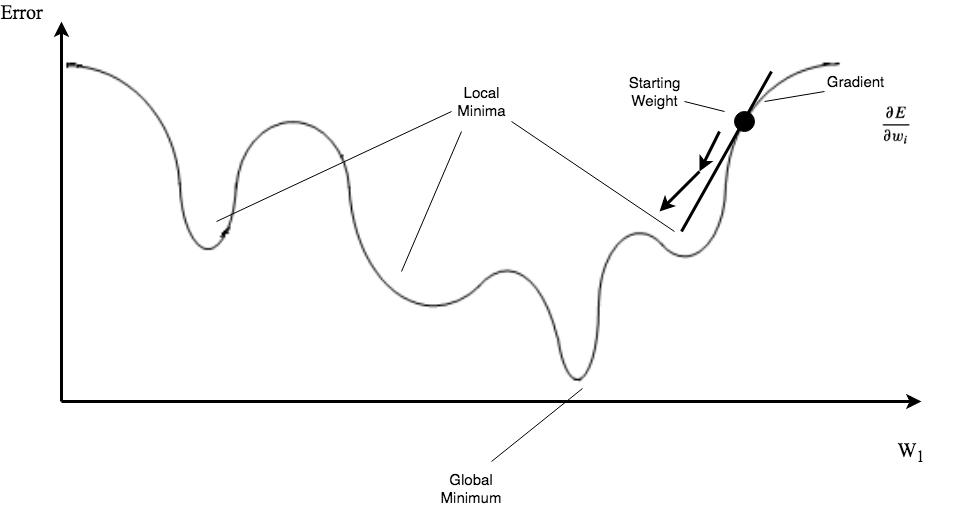
\includegraphics[max width=\textwidth]{gradient-descent}
	\caption{Weights are updated to minimize the error produced by the cost function in an effort to reach the global minimum.}
	\label{fig:gradient-descent}
\end{figure}

\subsubsection{Stochastic Approximation and Batch SGD}

Gradient descent can be considered a strategy for searching through a hypothesis space provided that the error can be differentiated with respect to the hypothesis parameters like the weights of a perceptron. There are two drawbacks however. First, gradient descent tends to be slow in converging on to a local minimum. Second, in more complex hypothesis spaces where there are many local minima, there is no guarantee that the gradient decent will reach the global minimum. There are two ways we can modify the gradient descent algorithm to optimize the learning process: stochastic approximation and batch stochastic gradient descent\cite{Mitchell}.

Instead of running all training examples through the gradient descent algorithm before summing up the error and calculating the weight update, with stochastic gradient descent we calculate the error and perform the weight updates after each training example is introduced to the network. Equation \ref{eq:weight-update} will therefore be replaced by:
\begin{equation}
\Delta w_i = \eta (t_d - y_d) (x_{id})
\end{equation}
This approach can take longer to train a network but has the advantage of adding a stochastic component due to the individual weight changes made for each example. This can increase the likelihood that the algorithm moves out of a local minimum and converges to a more optimal set of weights.\cite{Mitchell}.

A slight modification to the stochastic gradient descent (SGD) approach is to use batch SGD. With batch SGD, instead of updating the weights after every training example, the weights are updated after a batch of examples are introduced to the network. The batch size can vary and can have a significant impact on the training outcome. Using batches of examples maintains some of the speed up of the original gradient descent approach while also retaining the stochastic weight changes that can lead to better models. Batch SGD is used extensively in the experiments presented in Chapter 4.

\subsubsection{Adam Optimizer}

The learning rate is an important hyper parameter that can speed up the learning process when increased. However, higher learning rates can prevent the gradient descent algorithm from reaching a desired minimum in the hypothesis space, especially when the current gradient is close to that desired minimum. One modification that can be made is to introduce a learning rate decay parameter. With learning rate decay, after every epoch (a single iteration where all training examples are introduced to the network) the learning rate is decreased by a factor defined by the decay rate. This makes training faster early in the gradient descent where it is highly unlikely the algorithm will skip a desired minimum and prevents this from happening the closer we converge onto a minimum\cite{Mitchell}.

Other gradient descent techniques introduce a momentum factor to achieve the same goal. This momentum factor prevents the descent algorithm from changing direction too fast. This allows the algorithm to skip smaller shallow local minimums and also to continue down the slope faster when there is no change in gradient\cite{Mitchell}.

Some gradient descent techniques that have grown in popularity over the past decade take learning rate adaptation a step further. The Adam optimizer is one such algorithm that is an extension of the stochastic gradient descent. With Adam optimizer, every weight in the model has its own learning rate. This allows the algorithm to find a solution in a hypothesis space with sparse gradients (where the majority of weights are zero) such as those exhibited by computer vision problems\cite{DBLP:journals/corr/KingmaB14}.

Adam also uses moment to adapt each learning rate based on the current gradient of the parameter in question. Like momentum based techniques, moment allows the algorithm to go down the slope faster when there is little change in the gradient. However, this is done by adapting the learning rate instead of adding an additional factor. Specifically, Adam calculates an exponential moving average for the gradient and the square of the gradient. The learning rate is changed based on these averages and beta1 and beta2 values given as parameters to the optimizer\cite{DBLP:journals/corr/KingmaB14}.  Adam optimizer uses the following parameters with the following recommended values:
\begin{itemize}
	\item Alpha is the initial learning rate and is set to $0.001$
	\item Beta1 the rate by which the exponential moving average is decayed and is set to $0.9$
	\item Beta2 is the rate by which the exponential moving average  of the square of the gradient is decayed and is set to $0.999$
	\item Epsilon is a factor that prevents division by zero  and is usually set to $10^{-8}$
\end{itemize}	

The Adam optimizer is more efficient than other techniques that use a separate learning rate for each parameter. It also allows converging to a solution in the hypothesis space much faster than typical stochastic gradient descent\cite{DBLP:journals/corr/KingmaB14}. For these two reasons, the experiments conducted as part of the research presented in this thesis use the Adam optimizer exclusively as implemented in the TensorFlow library.


\subsection{Feed Forward Neural Networks} \label{sec:background-artificial-neural-networks-feed-forward-neural-networks}

A single neuron is limited to only discovering linear decision functions as show in Figure \ref{fig:separation-surface}(a). However, many real world problems are too complex to be modeled using a linear function (see Figure \ref{fig:separation-surface}(b)). Instead, individual neurons can be combined together into several layers to form a topology known as a feed forward network like the one shown in Figure \ref{fig:feed-forward}. Feed forward networks are composed of one or more fully connected layers, an output layer and zero or more hidden layers\cite{Mitchell}. By increasing the complexity of the network, the number of weights increases and in turn the separation surface (decision function) the model is able to represent also increases in complexity. This allows the neural network to effectively perform more difficult tasks\cite{Bengio07scalinglearning}.

\begin{figure}[t]
	\centering
	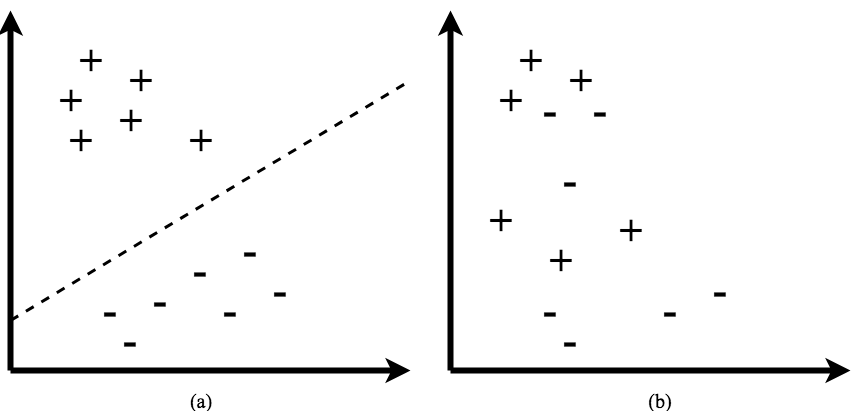
\includegraphics[max width=\textwidth]{separation-surface}
	\caption{A linear decision function (a) can not represent models that can solve more complex problems (b).}
	\label{fig:separation-surface}
\end{figure}

Feed forward networks are trained in the same way as single perceptrons, by running the training dataset through the network and minimizing the error between the outputs and the expected results. Gradient descent is also used to find the approximate weights that will minimize the value of the cost function. However, applying gradient descent to feed forward networks is slightly more involved given the complex nature of the models.\cite{Le15atutorial}.

\begin{figure}[t]
	\centering
	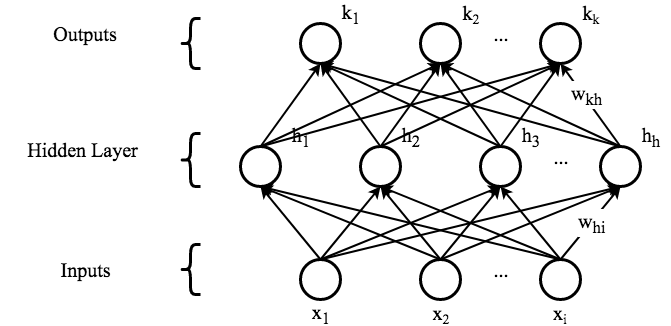
\includegraphics[max width=\textwidth]{feed-forward}
	\caption{A feed forward neural network with a single hidden layer.}
	\label{fig:feed-forward}
\end{figure}

\subsubsection{Backpropagation Algorithm}

The Backpropagation Algorithm is used to apply gradient decent to the individual units of the network\cite{Mitchell}. Initially the network weights are set to random values. Then for each training example, the backpropagation algorithm goes through two stages. First the input is propagated forward and the output $o_u$ of every unit $u$ is calculated. Next comes the backpropagation part where errors are propagated backwards through each layer and new weights are calculated.

For each output unit $k$ an error term $\delta_k$ is calculated
\begin{equation}
\delta_k \leftarrow y_k (1 - y_k)(t_k - y_k)
\end{equation}
where $y_k$ is the actual output of the output unit $k$ and $t_k$ is the target for output unit $k$. Then the error $\delta_h$ for each hidden unit $h$ is calculated
\begin{equation}
\delta_k \leftarrow y_h (1 - y_h) \sum_{k \in outputs} w_{kh} \delta_k
\end{equation}
where $y_h$ is the output from hidden unit $h$ and $w_{kh}$ is the weight of the connection between the hidden unit $h$ and the output unit $k$. Finally the weight of the connection from unit $i$ to unit $j$ is updated using the following update rule
\begin{equation}
w_{ji} \leftarrow w_{ji} + \eta \delta_j x_{ji}
\end{equation}

\subsubsection{Activation Functions}

\begin{figure}[t]
	\centering
	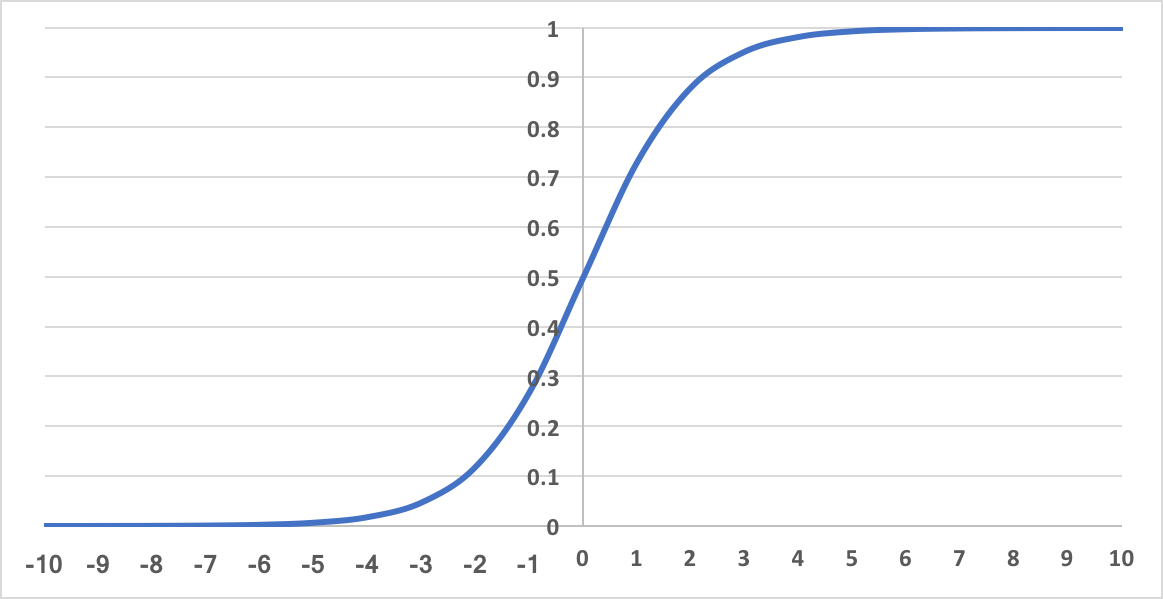
\includegraphics[max width=\textwidth]{sigmoid}
	\caption{A graph depicting the logistic form of the sigmoid function.}
	\label{fig:sigmoid}
\end{figure}

The choice of activation function limits how well the model can represent the underlying problem. In addition, the activation function determines the chain rule that is used to derive the gradient descent update rule. Here we discuss some variations of activation functions and how they affect the ability of neural network models to represent the desired target function. Some functions are best used for output layers because they model a probability distribution like the linear, sigmoid and softmax activations. On the other hand, rectified linear units and hyperbolic tangent activations are used in hidden layers because their derivatives remain generally high. This helps avoid the vanishing gradient problem discussed in Section \ref{sec:background-sequential-models-long-short-term-memory-units}\cite{Goodfellow-et-al-2016}.

Linear units model Gaussian distributions and use a linear activation function where the sum of the weighted inputs is output without transformation. The following formula shows how the output of a linear unit is calculated:
\begin{equation}
\vec{y} = W\vec{x} + b
\end{equation}
Linear activations make it easier for the gradient descent optimizer to find a more desirable minimum. However, they do not represent nonlinear functions very well\cite{Goodfellow-et-al-2016}.

If the output of a neural network involves predicting a binary value, like performing classification with two classes, sigmoid activations can be used. Sigmoid units can be viewed as a linear layer that is then transformed using the sigmoid function\cite{Goodfellow-et-al-2016}. Figure \ref{fig:sigmoid} shows a graph of a sigmoid function and equation \ref{eq:sigmoid} shows the formula for the sigmoid activation function.

The final output activation is known as a softmax activation. These types of units are appropriate for modeling tasks that have an output which is a probability distribution over a discrete variable, for example, a classification problem where the classes are mutually exclusive. Like the sigmoid activation, the softmax activation is a linear layer that is transformed using the softmax function\cite{Goodfellow-et-al-2016}. The following is the softmax function:
\begin{equation}
softmax(z) = \frac{e^z}{\sum{e^z}}
\end{equation}

\begin{figure}[t]
	\centering
	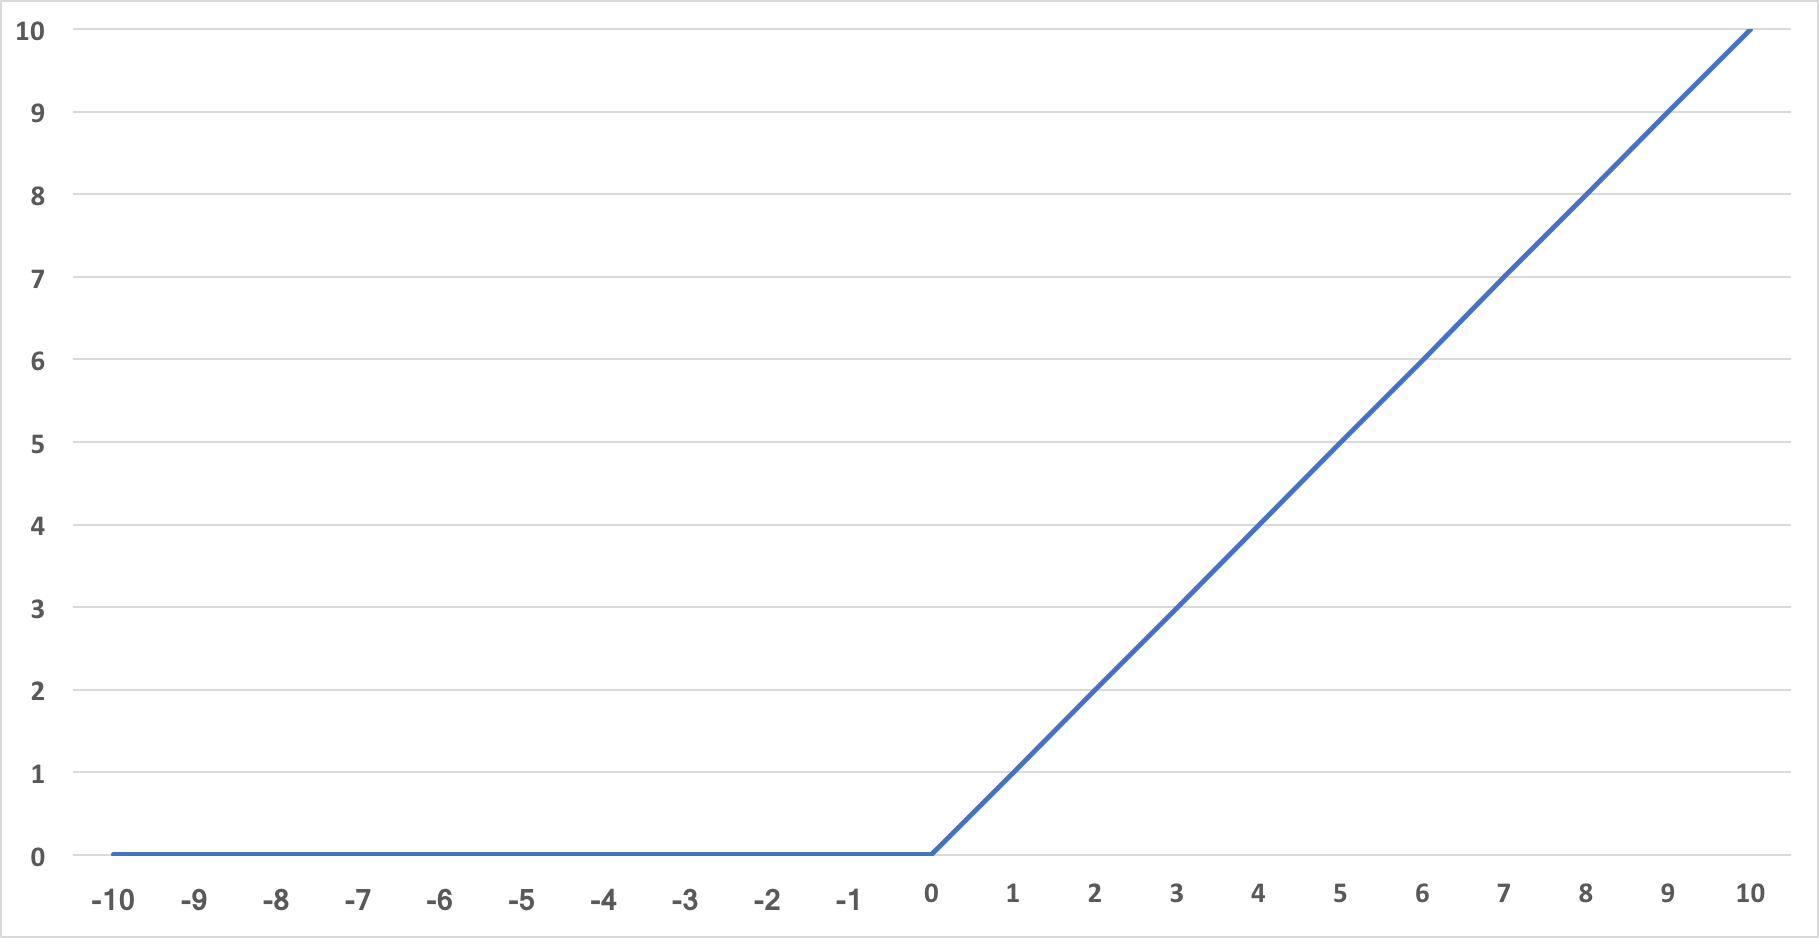
\includegraphics[max width=\textwidth]{relu}
	\caption{A graph of the rectifier function.}
	\label{fig:relu}
\end{figure}

The hyperbolic tangent activation and the rectifier activation are the two most common activation functions in hidden layers. The rectifier is similar to linear activation in that it is easier for gradient descent and also by eliminating values below zero, the gradients remain fairly high which is useful in rapid search for a solution hypothesis \cite{Goodfellow-et-al-2016}. Figure \ref{fig:relu} shows a graph of the rectifier function and the following is the formula for the activation of a rectified linear unit (a neuron with rectifier activation):
\begin{equation}
\label{eq:relu}
y(z) = max\{0, z\}
\end{equation} 

\subsubsection{The Problem of Overfitting}

\begin{figure}[t]
	\centering
	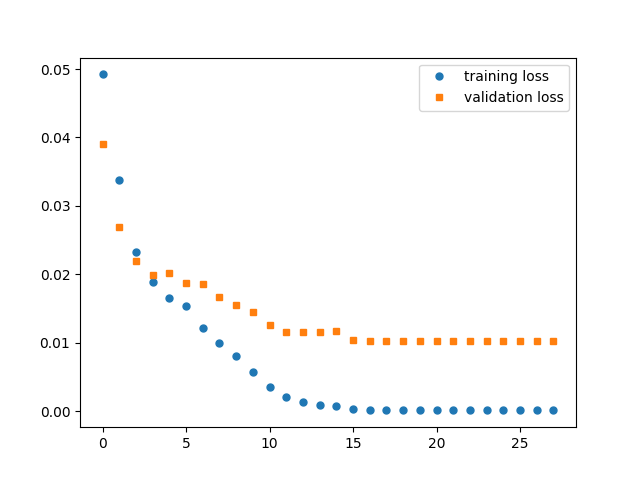
\includegraphics[max width=\textwidth]{overfitting}
	\caption{Comparison of training (circles) and validation (squares) loss over 30 epochs. At the 12th iteration the validation loss stops improving whereas the training loss continues to improve, indicating that the model is starting to overfit.}
	\label{fig:overfitting}
\end{figure}

An important goal of backpropagation is to find a representation that ``fits" the set of training examples and at the same time generalizes to yet unseen data points. Figure \ref{fig:overfitting} shows two graphs that depict the value of the mean squared error against the iteration number of a backpropagation run on a particular dataset. The graph shown in circles shows the errors resulting from the training set and the one in squares shows the errors resulting from the validation set. Notice that the errors from the training set continues to decrease as training proceeds, whereas the errors from the validation set decrease initially but start to stall around the twelfth iteration. This happens because, at the twelfth iteration, the backpropagation algorithm starts to overfit to the training dataset and fails to accurately generalize to the unseen dataset. The weights of the network fit to nuances of the training data that are not representative of the true function. Overfitting is a problem that should be avoided in order for the learning algorithm to create the layers of abstract features that can be used to represent the decision function\cite{Mitchell}.

Using a validation dataset while training is an important mechanism used to prevent backpropagation from overfitting. The validation dataset is independent from the training set and is applied to the model after every epoch. The learning system maintains two copies of the weights of the neural network. One copy holds the weights of the current iteration and the other copy holds the weights of the iteration that performed best on the validation set. When backpropagation stops performing better on the validation set, the best set of weights are returned as the hypothesis learned\cite{Mitchell}.

\subsubsection{K-Fold Cross Validation}

When testing the accuracy of trained neural networks, it is important that the dataset used for testing include a variety of examples that are representative of the overall task. However, with limited datasets, it is difficult to acquire test data that is representative of the problem and therefore it throws into question the effectiveness of the trained model\cite{Goodfellow-et-al-2016}.

Cross-validation is instead used when working with smaller datasets to allow the entire dataset to be used as a test set. With k-fold cross-validation, the dataset is split into k number of non-overlapping subsets. Then training is repeated k times; each time one of the subsets is set aside for testing and the other $k-1$ subsets are used for training. The accuracy score of each iteration is then averaged to produce the overall accuracy of the model. This ensures that the entire dataset contributes to the test set\cite{Goodfellow-et-al-2016}.

In our experiments presented in Chapter 4, we deliberately use small datasets to emulate the difficulty an individual human learner encounters when learning on their own. However, this introduces uncertainty in the accuracy scores obtained from training these models\cite{Goodfellow-et-al-2016}. We therefore use k-fold cross-validation to mitigate this issue.

\subsection{Deep Learning} \label{sec:background-deep-learning}

One of the factors that determines the effectiveness of neural network models is how the features that define the model's inputs and outputs are represented. For example, to construct a model that learns to classify objects in an image, the images would traditionally be pre-processed to extract certain features like edges before being fed into the neural network model. The quality of the feature engineering process significantly affects the outcome of the classification. Certain application domains do not have automated algorithms that can pre-process inputs, in which case feature engineering must be done manually\cite{Goodfellow-et-al-2016}.

To avoid the effort and error introduced by manual feature engineering, machine learning models are adapted to learn feature representations. This usually results in models that perform better than the ones that depended on manually specified features. The ability of these machine learning models to identify the important aspects of the application domain, such as facial recognition, depend on the ability of such models to disentangle the factors of variation that comprise the problem\cite{Bengio:2009:LDA:1658423.1658424}.

This process of separating the important factors from those that are not is considered difficult. In order to capture the complexity of such tasks, we construct representation learning models that are several layers deep. Constructing models in such a layered topology allows the models to represent the application domain in terms of a hierarchy of concepts, with each concept defined through its relation to simpler concepts\cite{Goodfellow-et-al-2016}. Each layer represents the model's understanding of a particular level of abstraction with each level being more abstract than the layer below\cite{Bengio:2009:LDA:1658423.1658424}. This borrows from the fact that our nervous system processes sensory input via a multi-layer hierarchy of neurons\cite{DBLP:journals/corr/abs-1203-2990}. For example, a model that can be used to identify objects in an image can be constructed in several layers. One layer learns to identify edges, the next layer learns to identify simple shapes all the way up to the final layer (output layer) that makes the actual classification.

Figure \ref{fig:feature-representation-learning} shows an example of what the weights of each layer of a deep neural network would learn to represent. Raw pixels are presented as input to the network, the first hidden layer then detects the edges in the image, the second layer detects parts of an object and the final hidden layer detects the object. The model then outputs the classification of what it ``sees" in the input image.

\begin{figure}[t]
	\centering
	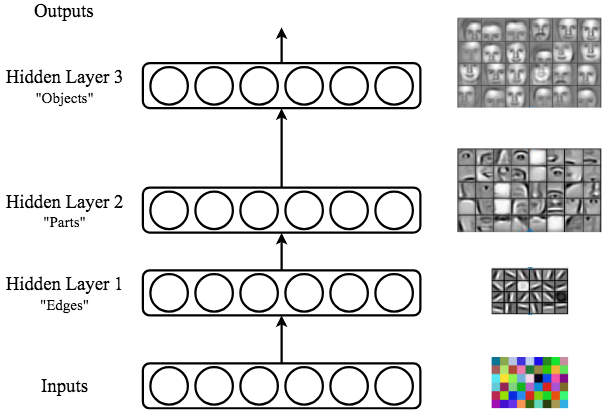
\includegraphics[max width=\textwidth]{feature-representation-learning}
	\caption{Deep feed forward neural network learning to classify objects in an image. Each layer learns to represent a level of abstraction that is more high level than the layer below.}
	\label{fig:feature-representation-learning}
\end{figure}

\subsubsection{The Depth-Breadth Tradeoff}

Besides increasing the representational power of neural network models, empirical evidence also shows that by adding more layers to the neural network architecture the efficiency of the model is also improved. 

The computational complexity of both the feed forward phase and the backpropagation phase of a feed forward neural network is dependent on the number of parameters (weights) that define the model. By having an architecture that is as compact as possible, but at the same time has sufficient complexity to represent the target function, we reduce the required number of weights and therefore have a better performing model.

Bengio 2009 discusses that if a function can be compactly represented by a deep architecture, it might need an exponentially large architecture to be represented by an insufficiently deep one\cite{Bengio:2009:LDA:1658423.1658424}. Therefore, deep architectures help in discovering compact architectures that significantly reduce the computational complexity of the models.

\subsubsection{GPU Training}

The accuracy of trained neural network models depends on the number and variety of the training examples provided. The more factors of variation the problem exhibits the more examples the model will need in order to capture the complexity of the problem. It is therefore important to develop methods to improve the speed of training, especially for difficult problems. One way to accomplish that is by using parallelism. This refers to using more than one processor to train a single model.

There are two forms of parallelizing neural networks. The first is model parallelism, which refers to partitioning the neurons that make up the model onto several processors. Communication is needed so that the outputs of one partition can be fed into another partition. The second type of parallelism is called data parallelism. Each machine holds a copy of the model and the training data is divided among the copies. Each copy is trained independently and then the weight values are integrated after training\cite{Le15atutorial2}.

Many off the shelf computers incorporate Graphics Processing Units (GPUs) that support General Purpose GPU computing (GPGPU). GPUs can have hundreds and sometimes thousands of processing cores collectively allowing for parallel computing. This makes it convenient and affordable to parallelize machine learning. Some machine learning libraries like TensorFlow support running models on GPU powered machines. In this research, we take advantage of GPUs to run our experiments.

\subsubsection{Sequential Models} \label{sec:theory-approach-methodology-sequential-models}

\begin{figure}[t]
	\centering
	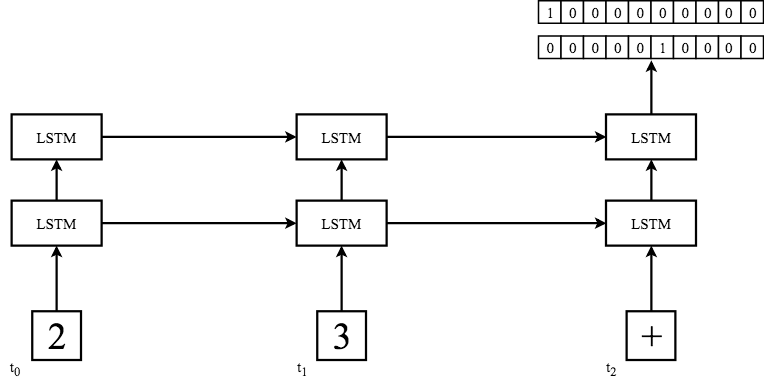
\includegraphics[max width=\textwidth]{sequential-model-arithmetic}
	\caption{A deep LSTM network that accepts a sequence of two operands and learns to perform addition on them.}
	\label{fig:sequential-model-arithmetic}
\end{figure}

When humans perform arithmetic operations, like addition, they tend to read an operand, followed by an operator, followed by another operand and then they perform the operation and produce an output. This approach to arithmetic is sequential in nature and depends on our ability to retain a representation of the operands in our minds as we read them, before we perform the operation. Given that recurrent neural networks are better suited to modeling these kinds of sequential processes, as discussed in Section \ref{sec:background-sequence-modeling}, we therefore opted to using recurrent neural networks for our experiments.

Figure \ref{fig:sequential-model-arithmetic} shows how the arithmetic expression 2 + 3 = 5 can be modeled using recurrent neural networks. On each time step the model accepts a 28x28 image of a handwritten digit from the MNIST dataset. On the last time step the model receives the operator, again in the form of a 28x28 image, and produces an output which is the result of performing the operation on the two operands. The result is represented using a pair of one-hot vectors, one vector represents the least significant digit of the result and the other represents the most significant digit of the result. Notice that we provide the operator on the final time step as opposed to the middle time step. This is because we use reverse Polish notation (RPN) when presenting the operations to the neural networks.

\paragraph{Reverse Polish Notation}

The reverse Polish notation (RPN) is a notation used to depict arithmetic expressions without the need for parentheses to indicate precedence. Unlike traditional mathematical notation where the operands of a binary operator are placed on the left and right of the operator, in RPN both operands precede the operator. The expression
\begin{gather*}
	(7 + 5) - 2
\end{gather*}
would be expressed as
\begin{gather*}
	7\ 5\ +\ 2\ -
\end{gather*}
As long as the operations have a non-variable number of operands, any arbitrarily long sequence of operations can be represented in RPN\cite{wiki:reverse-polish-notation}.

Early stack based computer models based on the work of Dijkstra and Bauer utilized RPN to reduce memory access while evaluating mathematical expressions\cite{wiki:reverse-polish-notation}. Hence, we believe that using RPN to train neural networks to perform arithmetic operations would reduce the complexity of the problem, making it easier to investigate the core hypothesis of this thesis and focus on contrasting the models' accuracy due to the presence of symbols or lack thereof instead of worrying about other factors.

\section{The Problem of Local Minima} \label{sec:background-problem-local-minima}

Combining many layers of features together to form a neural network may increase the expressiveness and accuracy of the model, however, it adds challenges to the training process. A major challenge for the training algorithm is to search for a global minimum in the hypothesis space, given the presence of many local minima in hypothesis spaces with lower dimensions\cite{Larochelle:2009:EST:1577069.1577070} and the presence of many saddle points and plateaus in higher dimensions\cite{DBLP:journals/corr/DauphinPGCGB14}. Figure \ref{fig:gradient-descent} depicts the training set loss as a function of the weights. The complex topology of the feed forward network adds regions in the loss function that act as local minima. In the context of a small dataset, this makes it more likely for the backpropagation algorithm to converge the weights to one of these local minima instead of the desired global minimum\cite{Larochelle:2009:EST:1577069.1577070}. Overcoming this difficulty in training can be achieved by increasing the number of training examples used. Other techniques involve pre-training the network using unsupervised learning first before using the network as a classifier as is the case with deep belief networks\cite{Larochelle:2009:EST:1577069.1577070}.

When comparing machine learning to how we as humans learn, we find that humans also suffer for the presence of effective local minima that hamper their ability to learn from small datasets\cite{Larochelle:2009:EST:1577069.1577070}. In the next chapter, we present our theory that considers how this problem can be overcome in artificial neural networks by introducing a symbolic channel. This symbol channel emulates how the concise knowledge shared by human learners helps individual humans overcome otherwise impoverished training data. The symbolic channel introduces bias that favors regions of the hypothesis space avoiding local minima and allowing the gradient descent process to converge to a more suitable minimum.

\section{Summary} \label{sec:theory-summary}

This chapter presented our basic hypothesis. The theory states that individual human learners struggle to learn new concepts through experimentation alone when the number of examples provided to them is limited. However, through interaction with other learners, common symbols for noisy concepts are shared that allows the learner to overcome the challenges in developing accurate models. We hypothesize that the introduction of such a symbolic channel to an artificial neural network model can also help the model achieve higher levels of accuracy when training with an impoverished dataset.

We also proposed a problem domain to validate this hypothesis, namely to teach artificial neural network models to perform arithmetic on images of handwritten digits. We first explained that the process of learning arithmetic operations can be modeled using sequential neural network architectures. We then presented two methods of supplying symbolic information to these models. Next, two theories were discussed on the role the symbols play in guiding the learning system towards discovering an optimum solution to the problem. Finally, we introduced a new form of symbolic representation, that of temperature encoding, that we believe will capture all aspects of learning to perform arithmetic and will therefore produce the best results. 
    \chapter{Theory} \label{sec:theory}

In Section \ref{sec:background-problem-local-minima} we discussed how deep neural networks suffer from the problem of local minima. Due to the complex nature of deep architectures, the error surface includes many peaks and valleys. The gradient descent algorithm is therefore more likely to converge on to one of these local minima as opposed to the desired global minimum\cite{Larochelle:2009:EST:1577069.1577070}. Typically, this problem is overcome by providing more training examples with more variety to the learning algorithm. In contrast, human learners build on the knowledge they accumulate over their lifetimes and therefore related tasks require fewer examples to learn\cite{Thrun1998}. 

Individuals in a society can also benefit from the knowledge accumulated over generations through language that can symbolize this knowledge. By sharing these symbols, learning in humans becomes less expensive and more effective\cite{DBLP:journals/corr/abs-1203-2990}. The goal of our research is to demonstrate that this form of symbolic knowledge transfer can be emulated in artificial neural networks to improve the accuracy of training.

This chapter starts by presenting our theory of learning with symbols and how it relates to deep neural networks and multi-task learning. We then discuss previous work that provided the inspiration to our approach. Finally, we outline the problem domain and the methodology we propose to empirically test our theory.

\section{Hypothesis} \label{sec:theory-hypothesis}

Chapter 1 discussed how it can be expensive and risky for an individual human learner to acquire a clear understanding of their environment purely through experimental trial and error. We believe that learning in individual humans is hampered by challenges of observing sufficient numbers of training examples, but accelerated by the occasional sharing of knowledge in the form of symbols.

Human societies develop languages and communication techniques that allow individuals to share knowledge with one another in a clear and concise manner\cite{DBLP:journals/corr/abs-1203-2990}. This shared knowledge introduces inductive bias in the way humans think and in turn, helps the individual human learner gain a better understanding of the problem or environment\cite{Thrun1998}. This understanding allows the learner to develop more optimal solutions. We call this shared knowledge, symbolic knowledge or simply symbols.

Artificial neural networks also experience difficulty in discovering the desired decision function when training with a limited dataset. This is due to the existence of many local minima in the error function. Just as humans overcome this difficulty with the aid of clear symbols, through interactions with other individuals, we hypothesize that the introduction of a clear symbol channel to an artificial neural network will also help the artificial model overcome the challenge of training with a small dataset and improve the model's overall accuracy on test data.

In the context of this research, \textbf{symbols} are defined as \textit{clear, concise and consistent external representations of a concept that captures its key regularities and is meant to be shared between learning agents}. For example, when considering handwritten digits like those found in the MNIST dataset, discussed in \ref{sec:theory-approach-the-mnist-dataset}, there are a wide variety of examples of the same digit. The existence of these many variations makes handwritten digits noisy and in order for a neural network to successfully classify these inputs, the network must learn the important features that are common among all variations of each digit and filter out the noise. In contrast, a symbol for a concept shared by learning agents, such as the digit ``2", must have a consistent representation that captures the key regularities of the concept. Examples of symbolic representations can be a one-hot vector or an image rendered using a standard font.

We believe that learning a concept task from noisy inputs can benefit from learning the same task from clear and consistent symbols of the same concept.  Representation created in the layers for mapping the symbolic inputs to outputs that correctly identify the concept can be used as a scaffold for mapping the noisy inputs to the same outputs. In this way, the weight updates associated with the symbolic inputs guide the backpropagation algorithm to areas of weight space that have fewer suboptimal local minima. The weight updates associated with the noisy inputs will piggy back on the movement along this trajectory because the gradient of the error with respect to the weights will be highest in this direction. This form of inductive bias results in a model that has a higher accuracy than if learned with only the noisy inputs.

\newtheorem*{symbolic-learninig-hypothesis*}{Hypothesis}

\begin{symbolic-learninig-hypothesis*}
	\label{hypothesis:symbolic-learninig-hypothesis}
	Similar to how individual human learners overcome the difficulties they encounter while learning a concept from an impoverished dataset, an artificial neural network can overcome the local minima problem by guiding the development of more beneficial internal representations through the use of shared symbols that capture the key regularities of the concept.
\end{symbolic-learninig-hypothesis*}

Our intention is not to discover the mechanism by which human learners use symbols to develop more accurate representations of concepts, rather it is to determine if the introduction of such symbols can assist machine learning systems in developing more accurate representations. We would like to determine how neural networks can take advantage of symbols, however if found, we will make no claim as to the same mechanism being part of human learning.

\subsection{Multi-Task Learning} \label{sec:theory-hypothesis-multi-task-learning}

The insight for our hypothesis comes from our understanding of multi-task learning. In multi-task learning, a deep neural network model is trained to learn several different but related tasks together\cite{silver2007context}. Section \ref{sec:background-deep-learning} introduced deep learning and explained how deep neural networks are constructed from several layers of artificial neurons that learn levels of abstract representation of the input values. When learning multiple tasks, certain abstractions are shared among the different tasks, therefore reducing the overall number of training examples that are needed to learn any one task.

By incorporating a clear symbol channel into our networks, the deep architecture has a better chance of developing useful abstract representations from the noisy inputs\cite{Bengio:2009:LDA:1658423.1658424}. Since learning using the clear symbols is easier than learning from the noisy inputs, these common abstractions will be discovered early in the training process making the ability of the network to converge on a solution much easier, therefore improving the effectiveness of training.

\section{Approach} \label{sec:theory-approach}

To demonstrate the validity of the hypothesis presented above, we constructed several deep neural network models that learn to do basic arithmetic operations (namely addition, subtraction, multiplication and division) on images of handwritten digits. When properly trained, using sufficient training examples, the models can be presented with images of handwritten digits sampled from the dataset, and perform an arithmetic operation using the values depicted in the images provided.

We use the MNIST dataset to train and test our models. The MNIST dataset is a set of images depicting handwritten digits that are commonly used by image processing researchers\cite{MNIST}. Each image represents a single digit. Section \ref{sec:theory-approach-the-mnist-dataset} provides further details on the MNIST dataset. Figure \ref{fig:noisy-mnist} shows examples of the handwritten digits used from zero to nine. We refer to this type of input as noisy since there is no consistent way for rendering each digit. 

\begin{figure}[t]
	\centering
	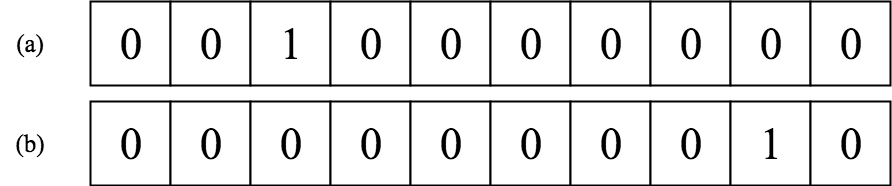
\includegraphics[max width=\textwidth]{one-hot-vector}
	\caption{Two one-hot vectors are depicted, (a) is a one-hot vector representing the integer two and (b) is another one-hot vector of the integer eight.}
	\label{fig:one-hot-vector}
\end{figure}

\begin{figure}[t]
	\centering
	
\includegraphics[max width=\textwidth]{noisy-mnist}
	\caption{Example of noisy handwritten digits sampled from the MNIST dataset.}
	\label{fig:noisy-mnist}
\end{figure}

The models are trained to output a set of one-hot vectors. One-hot vectors are vectors that have all their values set to zero except for the value corresponding to the category being represented, which is set to one. Figure \ref{fig:one-hot-vector}(a) shows an example of a one-hot vector for the number two and \ref{fig:one-hot-vector}(b) shows another example of a one-hot vector for the number eight.

Alongside the noisy handwritten digit inputs, the models are also provided a clear symbolic channel. This channel is analogous to the common language shared by human learners. The presence of symbolic inputs on this channel are controlled during training to investigate their effect on the accuracy of the network model when tested on noisy data only. Testing was performed without symbolic information to simulate the behavior of an independent agent that interacts with other agents. Our expectation is that models trained without the presence of symbols on an impoverished dataset will perform poorly on an independent test set. However, by gradually increasing the number of symbols provided during training, the model's performance should also gradually increase. Given the sequential nature of performing arithmetic operations, recurrent neural networks, like the one depicted in Figure \ref{fig:sequential-model-arithmetic}, specifically those based on long short-term memory (LSTM) units, will be used to investigate this theory. These networks will be discussed in detail in Section \ref{sec:theory-approach-methodology}.

Besides showing that the symbols help in improving the accuracy of the trained neural networks, we also want to establish an analogy between the role that symbols play in human learning and their role in improving the performance of artificial neural network models. In human learning, teachers use symbolic information in the form of examples that the learner is already familiar with to teach the learner a general method by which the learner can solve a specific problem.

Take teaching arithmetic to children for example. When teaching children how to add or divide numbers, a teacher uses objects the child is already familiar with, like apples for example, and shows the child how to relate a quantity of apples to a digit. The teacher then builds on that concept of quantity to show the learner how to add by counting one group of apples and then continue counting the other group, and how to divide by distributing the apples evenly into containers. Over time, the children gain the ability to generalize these techniques to quantities and numbers they have not encountered during learning. Symbols allow the learner to move beyond memorizing inputs and their corresponding outputs, to learn an actual algorithm that represents a general solution to the problem.

We would like to show that just as in human learning, clear symbols can expedite the learning process in artificial neural networks so as to more accurately perform arithmetic operations and provide a general solution to the problem. To show that this is possible, some of our experiments are trained on a subset of digit combinations. The independent test set is composed of combinations of digits that are not encountered during training. When the models perform well on the unseen combinations we can conclude that the artificial model has indeed learned the general arithmetic rule and is not simply doing pattern matching. 

Given the above, our goals are:
\begin{itemize}
	\item To show that it is possible to develop a deep recurrent neural network model that can learn to perform all four basic arithmetic operations (addition, subtraction, multiplication and division) more effectively with the presence of symbols than without.
	\item To explain the role that symbols play in teaching arithmetic to a machine learning system by showing that the neural network models are able to discover a principled algorithm as opposed to simply memorizing input and output patterns.
\end{itemize}

In the following sections, we describe the various network architectures and learning techniques that will be used in exploring this theory. Chapter 4 provides a detailed description of the empirical studies performed along with the results and a discussion.

\subsection{The MNIST Dataset} \label{sec:theory-approach-the-mnist-dataset}

All of our experiments use the MNIST dataset of handwritten digits. This is a database of images of handwritten digits along with labels indicating the values represented. Each digit is pre-processed so that the digit is normalized and centered in a 28x28 pixel image. The digits in the images all have the same scale and orientation. The dataset consists of 60,000 training examples and 10,000 test examples. MNIST is very popular among researchers that need to quickly test machine learning techniques since the dataset is pre-processed \cite{MNIST}. Figure \ref{fig:noisy-mnist} shows examples of MNIST digits from zero to nine.

\subsection{Multimodal Learning} \label{sec:theory-approach-multimodal-learning}

\begin{figure}[t]
	\centering
	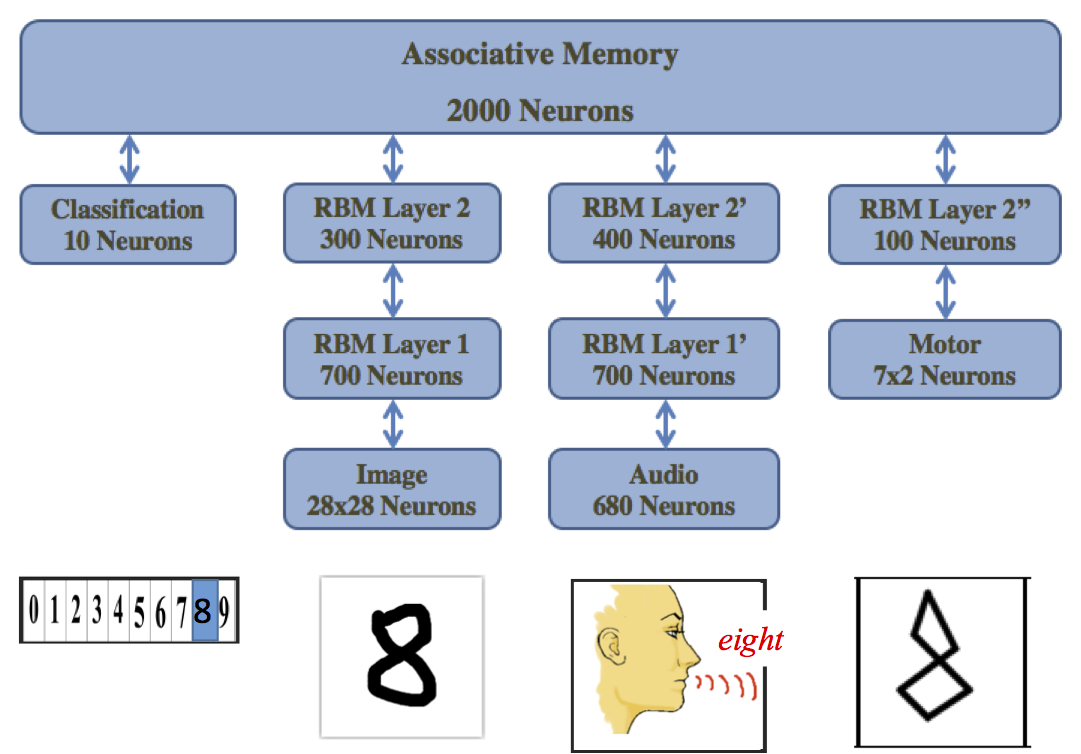
\includegraphics[max width=\textwidth]{multimodal-learning}
	\caption{A Multimodal neural network trained to communicate digits using several mediums. Each channel is modeled as a stack of Restricted Boltzman Machines connected to an associative layer\cite{iqbal2016scalable}.}
	\label{fig:multimodal-learning}
\end{figure}

Recent work by Iqbal and Silver (FLAIRS-2016 Best Paper Award)\cite{iqbal2016scalable} inspired by work by Hinton et al.\cite{Hinton:2006:FLA:1161603.1161605} and Srivastava et al.\cite{JMLR:v15:srivastava14b} has shown that it is possible to develop a multimodal deep learning system for learning a noisy handwritten digit using four sensor/motor channels (visual, audio, robotic, and symbolic) and an associative layer that ties all channels together.  After training, the presentation of a digit (sound, image, drawing) at the visible nodes of the model activates all other channels to create their associated reconstruction at their respective visible nodes. Each channel provides additional information that helps the other channels more accurately reconstruct the output. 

Figure \ref{fig:multimodal-learning} depicts the architecture that was developed as part of that work. Each channel is modeled as a stack of Restricted Boltzman Machines (RBM). A Restricted Boltzmann Machine is a generative neural network that can learn a probability distribution over its set of inputs. One important application of generative models is auto-encoding for feature engineering. Given a noisy input, an auto-encoder is able to extract a feature vector that is representative of the input based on the probability distribution being modeled\cite{pmlr-v5-salakhutdinov09a}.

\begin{figure}[t]
	\centering
	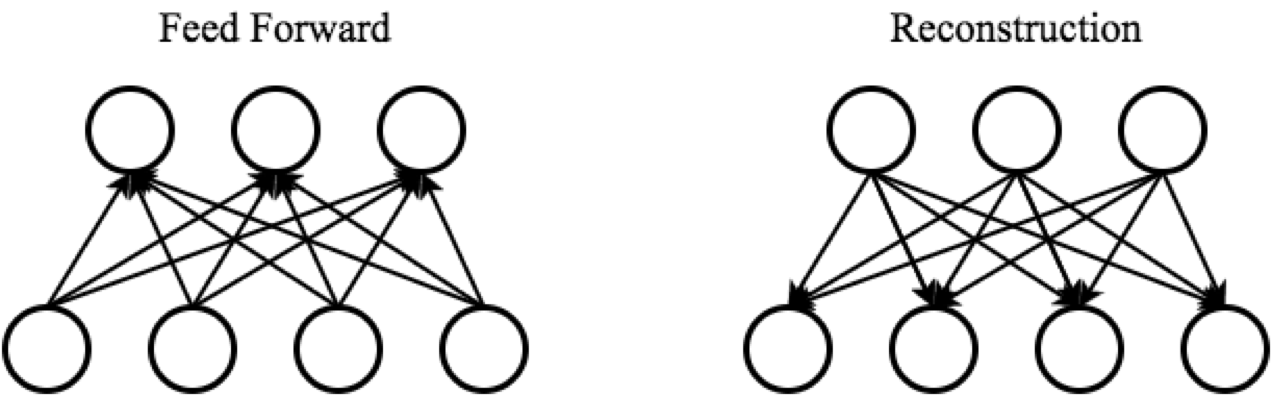
\includegraphics[max width=\textwidth]{rbm}
	\caption{An example of a Restricted Boltzman Machine showing the feed-forward pass and the reconstruction pass.}
	\label{fig:rbm}
\end{figure}

RBMs consist of an input layer and a hidden layer where the feature that represents the input is constructed. Training involves using the contrastive divergence (CD) algorithm to iteratively present the network with input examples, where an output is produced on the output layer during a feed-forward pass, and then the input is reconstructed back from that output. Figure \ref{fig:rbm} is a depiction of the architecture of an RBM showing the feed-forward and reconstruction passes. The goal of CD is to find an optimum set of weights that minimizes the reconstruction error. Contrastive divergence is an unsupervised process since there are no labels associated with the data. When fully trained, the output of RBMs is treated as a representation of the inputs that can be used in other machine learning tasks as is the case with deep belief networks\cite{Hinton:2006:FLA:1161603.1161605}.

The multimodal model developed by Iqbal and Silver\cite{iqbal2016scalable} learns to reconstruct the input presented to one channel on the other three channels each in their respective format (image, sound, robotic motion and symbol). The symbolic channel outputs the clearest signal as to which digit the multimodal deep learning system is ``thinking" about, given the input on the other channels. The symbolic channel also provides the clearest input for the other channels to generate the correct reconstructions at their visible nodes. This led us to a paper by Bengio\cite{DBLP:journals/corr/abs-1203-2990} that discusses the value of symbols and language in helping individuals learn concepts effectively without having to see all possible examples of that concept. This knowledge transfer in the form of symbols has a profound impact upon the development of our culture and the human species. 

Multimodal learning has inspired us to consider developing learning agents that learn to perform arithmetic operations using noisy channels but which can at times also receive concise information on a symbolic channel about the data on the noisy channels. The conjecture is that symbols are predominantly external communication tools that allow agents to share otherwise complex noisy concepts and in this way help them avoid local minima in model development. Clear symbols develop abstract representations that provide beneficial inductive bias during learning, therefore reducing the number of examples required to accurately learn a new concept.

\subsection{Methodology} \label{sec:theory-approach-methodology}

In this section we discuss the progression of our theory development. We provide a general overview of the neural network architectures that we are using as well as the rationale for using these architectures. There are three stages to the development of our theory. We start by describing the first stage which involves using sequential LSTM networks to perform the arithmetic operations on handwritten digits. We also discuss various techniques of supplying the symbols to our models and contrast the effectiveness of these techniques. Next, we discuss the second stage which attempts to explain the role that symbols play in improving the effectiveness of our models. Specifically, we would like to show that the networks that are trained using symbols are capable of discovering an algorithm that generalizes to all combinations of digits, instead of simply doing pattern matching, as is the goal presented above. Finally, we describe the third stage of theory development where a different representation of our symbolic channel produces the best results.

\input{theory/approach/methodology/sequential-models/sequential-models}

\input{theory/approach/methodology/symbol-channels/symbol-channels}

\input{theory/approach/methodology/pattern-matching-vs-learning-an-algorithm/pattern-matching-vs-learning-an-algorithm}

\input{theory/approach/methodology/temperature-encoding/temperature-encoding}

\section{Summary} \label{sec:theory-summary}

This chapter presented our basic hypothesis. The theory states that individual human learners struggle to learn new concepts through experimentation alone when the number of examples provided to them is limited. However, through interaction with other learners, common symbols for noisy concepts are shared that allows the learner to overcome the challenges in developing accurate models. We hypothesize that the introduction of such a symbolic channel to an artificial neural network model can also help the model achieve higher levels of accuracy when training with an impoverished dataset.

We also proposed a problem domain to validate this hypothesis, namely to teach artificial neural network models to perform arithmetic on images of handwritten digits. We first explained that the process of learning arithmetic operations can be modeled using sequential neural network architectures. We then presented two methods of supplying symbolic information to these models. Next, two theories were discussed on the role the symbols play in guiding the learning system towards discovering an optimum solution to the problem. Finally, we introduced a new form of symbolic representation, that of temperature encoding, that we believe will capture all aspects of learning to perform arithmetic and will therefore produce the best results. 
    \chapter{Empirical Studies} \label{sec:empirical-studies}

This chapter presents the empirical studies conducted to investigate and verify the theory and hypothesis laid out in the previous chapter. The objectives of these experiments are to show that deep recurrent neural networks can learn to perform basic arithmetic and that the presence of shared symbols improves the accuracy of these networks when trained using an impoverished dataset. Moreover, we aim to show that the symbolic information presented to the models during training perform the same role that the symbolic knowledge shared between human learners performs. We do this by showing that in the presence of symbols, artificial neural networks are able to discover an algorithm that generalizes to all instances of the problem.

Our experimentations are divided into three groups based on the overall objective of the experiments. The first set of experiments presented in Section \ref{sec:empirical-studies-sequential-models-experiments} aims to prove our hypothesis by comparing the effectiveness of recurrent neural networks trained in the presence of symbols with that of the same networks trained without symbols. The second experimental group described in Section \ref{sec:empirical-studies-explaining-the-role-of-symbols} is meant to explain the role that symbols play in improving a model's accuracy. Finally, Section \ref{sec:empirical-studies-temperature-encoding-experiments} presents  experiments that show how symbols allow the recurrent neural networks to learn an algorithm that captures a general solution to the problem of learning mathematical operations. 

We begin this chapter by providing a general overview of how the experiments are conducted and how the results are compared. Next, we describe the technology and environment on which we developed and executed our experiments. Then we present our experiments, laying out in detail the objective, methodology and results of each experiment. A discussion is provided after each experiment analyzing the results and comparing them to that of previous experiments. In the next and final chapter we provide a summary of the outcomes of our research and how it can be further developed.

\section{Experimental Process and Model Evaluation} \label{sec:empirical-studies-model-evaluation}

This chapter presents seven experiments that investigate the main hypothesis and objectives set out in Chapter 3. The experiments involve training recurrent neural network models, specifically those based on LSTM units to compare the effectiveness of two or more methods of training these networks. The methods are usually variations of training the models in the presence or absence of symbolic features. After the models are trained, they are then tested on independent test datasets to determine each model's accuracy. The accuracy is the percentage of the number of operations a trained neural network is able to successfully complete relative to the entire dataset. Models are compared based on their accuracies and the ones with the highest score are considered most successful at accomplishing their task.

The process of developing the models involves iteratively training the neural networks on a training set. Each iteration is called an epoch and after every epoch a validation dataset is applied to the neural network using the set of weights obtained so far in the training process. An optimum set of weights is always maintained and is replaced with the current set if the current set outperforms the older set on the validation data. Validation is used to prevent overfitting and to also determine when to stop training. The model is trained for a large predetermined number of epochs. However, a stopping condition is applied where, if the network fails to find a better set of weights than the current optimum after a set number of iterations, training is terminated and the current optimum weights are returned as the final trained model. Section \ref{sec:background-artificial-neural-networks} provides more details on training artificial neural networks.

Most experiments gather and present the following four metrics for each neural network model developed:
\begin{itemize}
	\item Mean Accuracy: After each model is fully trained the test set is applied to obtain the model accuracy. The training and testing of each model is repeated five times with a different distribution of training, validation and test data based on k-fold cross-validation where k is set to 5. The mean accuracy is then calculated and this becomes the accuracy score of the model.
	\item Standard Deviation: The standard deviation of the accuracies obtained from each training attempt is calculated. Standard deviation is used to verify the quality of the results by providing a measure of a model's variance. Too much variance can lower the confidence in the results. Standard deviation is used to calculate the remaining two metrics.
	\item Hypothesis Test: The p-value from a standard hypothesis t-test is used to determine the statistical significance of the results. Typically values less than 0.05 means that the null hypothesis is invalid and therefore the results support the theory being tested.
	\item 95\% Confidence Interval: The confidence interval is the statistical margin of error that is considered when comparing two or more results.
	We usually display the mean accuracy, standard deviation and p-value in tables and show the mean accuracy along with the 95\% confidence interval on graphs.
\end{itemize}

\section{Environment} \label{sec:empirical-studies-environment}

Here we describe the hardware and software environments that were used to develop, train and test the neural network models used in the experiments discussed later in this chapter. Typically, the amount of hardware resources needed increases with the size of our datasets\cite{Bengio07scalinglearning}. Since we are deliberately training these neural network models on limited datasets, common off the shelf laptop or desktop computers can be used to replicate these experiments.

All of our models were developed and trained on a laptop with the following specs:
\begin{itemize}
	\item Make and model: Apple MacBook Pro (Early 2015)
	\item CPU: 2.7 GHz Intel Core i5
	\item Memory: 8 GB 1867 MHz DDR 3
	\item Storage: 120 GB Flash Storage
\end{itemize}	
All experiments were validated using k-fold cross-validation where k is set to 5. This means that each experiment was repeated five times. The time it took to run each experiment varied depending on the type of dataset used. The combined average time for all five attempts of the experiments based on images of handwritten digits was around ten hours. The average time for the experiments based exclusively on symbols was about one hour.

With regards to the software technology used:
\begin{itemize}
	\item Python 2.7 is used to code the scripts that construct, train and test the neural network models.
	\item NumPy is a Python library that allows Python's numerical datatypes to represent real numbers with higher precision. It also extends the capabilities of Python's lists to allow for matrix manipulation. TensorFlow and Keras depend on NumPy for their internal workings.
	\item TensorFlow is a native library with a Python wrapper that allows programmers to express mathematical processes like matrix multiplication and gradient descent training in the form of a process graph which Tenserflow can then offload to either a CPU or GPU for execution. Expressing algorithms using process graphs allows the neural network architectures being developed to be abstracted from specific implementations that target CPU or GPU powered machines and therefore enables TensorFlow to optimize the underlying implementation based on the resources available.
	\item Keras is an API that provides neural network developers the ability to specify architectures as well as hyper parameters to TensorFlow without having to manually program these constructs from scratch. This allows researchers to experiment with their theories without worrying about the validity of their implementations.
\end{itemize}	

Alongside the above technologies, the following were also used to format and analyze the results:
\begin{itemize}
	\item Microsoft Excel is used to compile and analyze the results as well as generate the charts presented in the coming sections.
	\item PIL is a Python library that allows developers to generate images. The images included in the sections providing qualitative analysis of our models are generated using PIL.
\end{itemize}

\section{Sequential Models Experiments} \label{sec:empirical-studies-sequential-models-experiments}

In Section \ref{sec:theory-approach-methodology-sequential-models} we explained how basic arithmetic operations, namely addition, subtraction, multiplication and division, can be learned using sequential models such as recurrent neural networks. We also introduced two approaches to providing symbols to neural networks while training; explicit and implicit symbols. This first set of experiments applies this sequential modeling technique to our problem of learning with symbols. We also compare the accuracies of using the two different approaches to providing symbols we discussed earlier, explicit symbols compared to implicit symbols. The overall objective of these experiments is to validate our hypothesis.

\subsection{Experiment 1: Using Symbols to Improve the Effectiveness of Learning} \label{sec:experiment-1}

\subsubsection{Objective}

The goal of this experiment is to demonstrate the validity of our hypothesis by showing that the presence of a clear and concise symbolic representation of the input data improves the learning accuracy of the models developed. The symbols are analogous to the shared knowledge used by human learners to overcome the difficulty in learning from a limited number of noisy examples as discussed in Section \ref{sec:theory-hypothesis}. This first experiment deals with models trained to perform addition only. Later experiments will expand the dataset to include all four basic arithmetic operations.

\subsubsection{Method}

We developed five models based on recurrent neural networks, specifically those based on LSTMs, that learn to sequentially add images of handwritten digits (see Figure \ref{fig:noisy-mnist}). When properly trained the network models can be queried with a sequence of two images, each representing a single digit, followed by an image of the ``+" operator.  The network will output two one-hot vectors representing the estimate of the sum of the input digits. One-hot vectors have all their features set to 0 except for the feature corresponding to the value being represented which is set to 1.

Alongside the handwritten digit input channel, the networks also have a second input channel meant to receive only a standard set of symbols. In the case of numeric digits, the symbols are of the digits zero through nine clearly rendered in a standard font. See Figure \ref{fig:symbols} for the symbolic images used in the experiment. After the five models are trained, the test set is applied to compare the effect of the two approaches of providing symbolic information, mentioned in Section \ref{sec:theory-approach-methodology-sequential-models}, on the accuracies of performing the addition, to the cases of having no symbolic data and only symbolic data.

As discussed in Section \ref{sec:theory-approach-the-mnist-dataset}, the MNIST dataset of handwritten digits is used to train and test all the models developed for all our experiments. A limited subset is sampled from the larger MNIST dataset to create an impoverished collection of examples that are used to train and test our models. The dataset is composed of two single digit inputs followed by the operator. For each of the 100 two digit combinations, we randomly sample ten examples from the MNIST database. For example, the 0 + 0 combination has 10 different examples sampled, the 0 + 1 combination has another 10 examples and so on. This number was chosen because it impoverishes the dataset and also provides room for improvement when introducing symbols. In total, one thousand different input/output pairs are composed. Figure \ref{fig:dataset-examples} shows example combinations, each combination having one sample from the MNIST dataset. Constructing the dataset in that way ensures that there is sufficient balance of training and testing examples for each combination.

\begin{figure}[t]
	\centering
	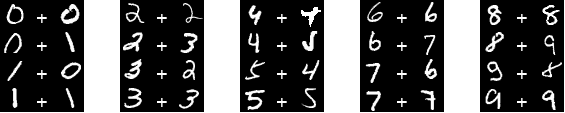
\includegraphics[max width=\textwidth]{dataset-examples}
	\caption{Some of the combinations of operands used for the experiment. Each combination shows only one sample selected from the MNIST dataset.}
	\label{fig:dataset-examples}
\end{figure}

A 5-fold cross-validation (discussed in Section \ref{sec:background-artificial-neural-networks-feed-forward-neural-networks}) approach is used to break down the dataset into a training, validation and test set such that for each combination of digits, six samples are used for training, two samples for validation and another two for testing. Since $k$ is set to 5, the training and testing of each of the five models is repeated five times, where the training, validation and testing samples for each combination are shuffled. The models for this experiment are exposed to all possible combinations of single digit operands during training. Some of the later experiments will only use a subset of the combinations for training and the rest for testing. After repeating the experiment five times for each model and recording the accuracies obtained from testing with the test sets, the mean accuracy and standard deviation for each model are calculated and used to compare the experiments graphically. A Hypothesis t-Test is also used to check the statistical difference of the means.

All networks trained have the same architecture, varying only in terms of the number of inputs. The architecture consists of two hidden LSTM layers, 512 units each, fully connected to an output layer, 20 units in length, composed of two one-hot vectors. This architecture was the result of trial and error and was found to have sufficient representation for the most difficult task at no detriment to the other tasks. The networks are trained using the Adam optimizer with the mean square error as the loss function and a learning rate of 0.001. Training is performed over 200 epochs (found to be sufficient for all methods) in batches of 100 and the set of weights performing best on the validation set is saved.  When evaluating the models, only noisy handwritten images are input and no symbol images are provided. The following paragraphs describe the five different architectures and training sets used.

\begin{figure}[t]
	\centering
	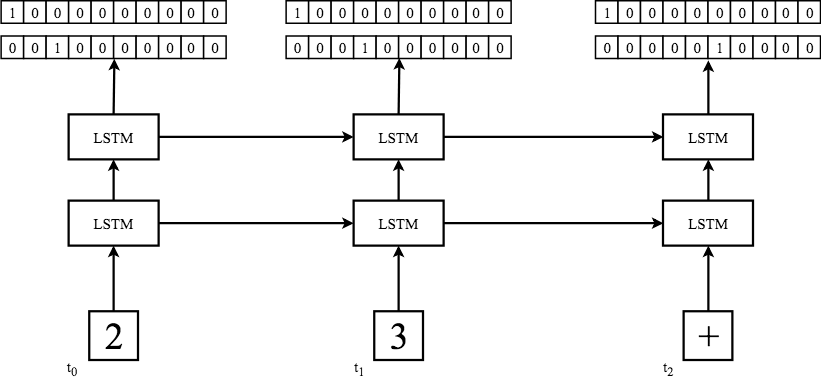
\includegraphics[max width=\textwidth]{sequential-model-symbols-only}
	\caption{Symbols Only (SO). A deep LSTM network that accepts a sequence of two operands and an operator. The operands are provided as the consistent symbol digits.}
	\label{fig:sequential-model-symbols-only}
\end{figure}

\paragraph{Symbols Only (SO).} The model learns to perform classification and addition using only the standard symbols (see Figure \ref{fig:sequential-model-symbols-only}). The input is a sequence of three 28x28 images, that are fed to the network one after the other. The first two images are that of the digits rendered clearly using a standard font. The third image is the plus operator. At each of the first two time steps the model is trained to classify the incoming digits producing two one-hot vectors representing the least and most significant digits of the input. Typically, the most significant digit will always be zero on these two time steps since we only use single digit inputs. When the plus sign is provided on the third time step, the network performs the addition operation, producing the result at the two one-hot vectors. The goal of training this model is to show that it is quite easy to do so using clear and consistent symbols.

\begin{figure}[t]
	\centering
	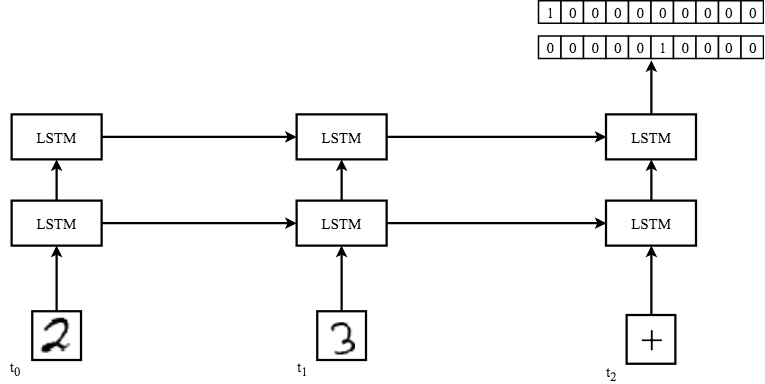
\includegraphics[max width=\textwidth]{sequential-model-noisy-only}
	\caption{Noisy Inputs Only (NO). A deep LSTM network that accepts a sequence of two operands and an operator. Only noisy operands are provided.}
	\label{fig:sequential-model-noisy-only}
\end{figure}

\paragraph{Noisy Inputs Only (NO).} The model learns to perform the addition using noisy handwritten digits without having to output the proper classes in the intermediate stages of the recurrent network (see Figure \ref{fig:sequential-model-noisy-only}). The input is a sequence of three 28x28 images, that are fed to the network one after the other. The first two images are that of noisy handwritten digit operands. The third image is the plus operator rendered in a standard font.  The goal of training the model using this method is to investigate the effectiveness of a network that is trained without the presence of symbols.

\begin{figure}[t]
	\centering
	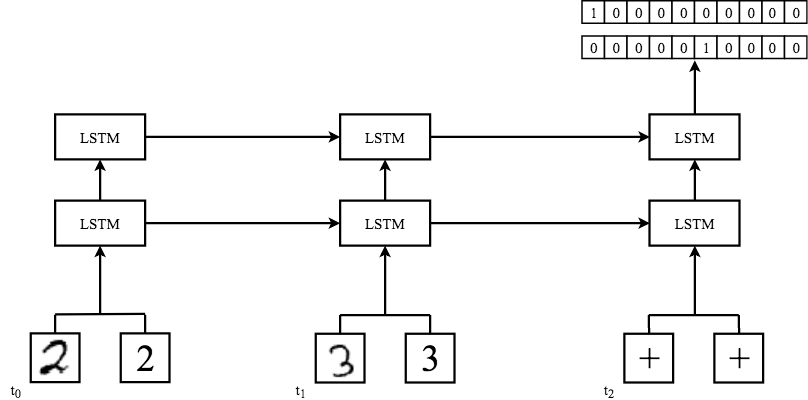
\includegraphics[max width=\textwidth]{sequential-model-symbols-noisy}
	\caption{Noisy and Symbol Inputs (NS). A deep LSTM network that accepts a sequence of two operands and an operator. Both the noisy operands and their corresponding symbolic information are provided alongside one another.}
	\label{fig:sequential-model-symbols-noisy}
\end{figure}

\paragraph{Noisy and Symbol Inputs (NS).} This model learns to perform addition without having to output the proper classes in the intermediate stages of the recurrent network (see Figure \ref{fig:sequential-model-symbols-noisy}). The input is a sequence of three pairs of 28x28 images, that are fed to the network one after the other. The first pair of images are of the first noisy handwritten digit operand and its matching standard symbolic digit. The second pair of images are for the second digit operand. The third pair of images are both the standard plus operator. The goal is to investigate the effect of introducing the clear symbol channel as an input (the explicit symbol) on the accuracy of the network.

\begin{figure}[t]
	\centering
	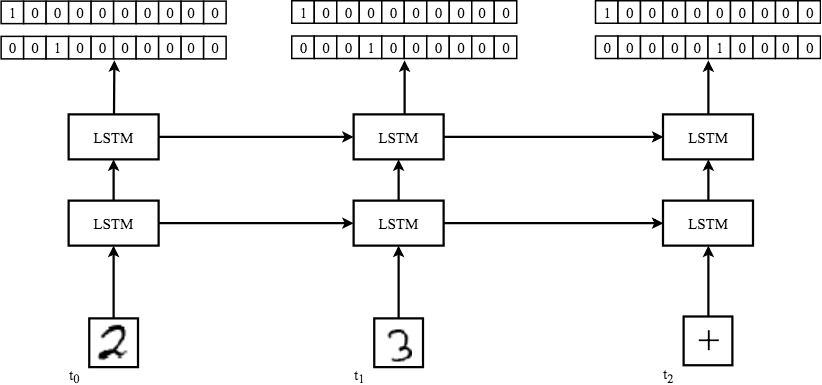
\includegraphics[max width=\textwidth]{sequential-model-noisy-classification}
	\caption{Noisy Inputs Only with Intermediate Classification (NC). A deep LSTM network that accepts a sequence of two operands and an operator. Noisy digits are provided as inputs and the network is trained to output the classes of each digit before performing the operation.}
	\label{fig:sequential-model-noisy-classification}
\end{figure}

\paragraph{Noisy Inputs Only with Intermediate Classification (NC).} The model learns to perform classification and addition on noisy digits only(see Figure \ref{fig:sequential-model-noisy-classification}). The input is a sequence of three 28x28 images, that are fed to the network one after the other. The first two images are that of handwritten digit operands. The third image is the plus operator. The model is trained to classify each incoming digit on each of the first two time steps by providing the class (as a one-hot vector) on the output during training and then perform the operation on the third time step. The goal is to investigate the effect of symbols on the accuracy of the network. However instead of using explicit symbols as inputs, the symbol is embedded in the LSTM context. By providing the classes of the handwritten digits while training, we believe that the network learns the symbolic information implicitly in the recurrent weights and then uses this information to aid in performing the mathematical operation.

\begin{figure}[t]
	\centering
	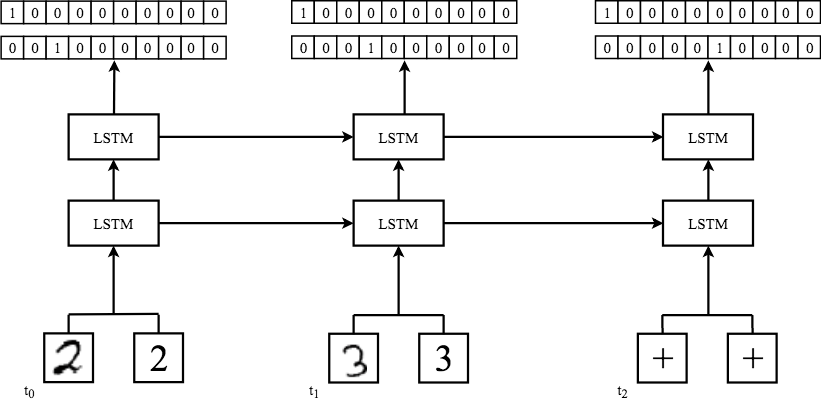
\includegraphics[max width=\textwidth]{sequential-model-noisy-symbol-classification}
	\caption{Noisy and Symbol Inputs with Intermediate Classification (NX). A deep LSTM network that accepts a sequence of two operands and an operator. Both the explicit and implicit symbols are provided.}
	\label{fig:sequential-model-noisy-symbol-classification}
\end{figure}

\paragraph{Noisy and Symbol Inputs with Intermediate Classification (NX).} This last model combines both methods of training used in NS and NC where the input includes the clear symbolic channel and the input classes are also provided on the output channel during training (see Figure \ref{fig:sequential-model-noisy-symbol-classification}). Here we investigate if a combination of the two methods of symbolic input improves on the individual approaches of the previous two methods.

\bigskip

While testing the trained Symbols Only (SO) model, we also test how well that model performs when tested on noisy handwritten digit inputs. We call this testing attempt \textbf{Symbols Tested with Noisy Inputs (SN)}. The objective is to see if training a recurrent neural network using only the idealized symbols will help the resulting model filter out the noise seen in the handwritten digits.

\subsubsection{Results}

\begin{table}[p!]
	\center
	\caption{A comparison of the mean accuracy and standard deviation of the models developed by the five methods. Also shown is the p-value of a hypothesis t-Test when compared to the NO method.}
	\label{tab:experiment-1-results-table}
	\begin{tabular}{ |c|c|c|c| } 
		\hline
		Method & Accuracy (\%) & Standard Deviation  & p-value, t-Test with NO Method\\ 
		SO & 100 & 0 & NA\\ 
		SN & 32.73 & 6.9 & NA\\
		NO & 60.16 & 4.5 & NA \\ 
		NS & 82.63 & 3.7 & 0.00317\\ 
		NC & 84.20 & 2.1 & 0.00102\\ 
		NX & 85.20 & 2.7 & 0.00043\\ 
		\hline
	\end{tabular}
\end{table}

\begin{figure}[p!]
	\centering
	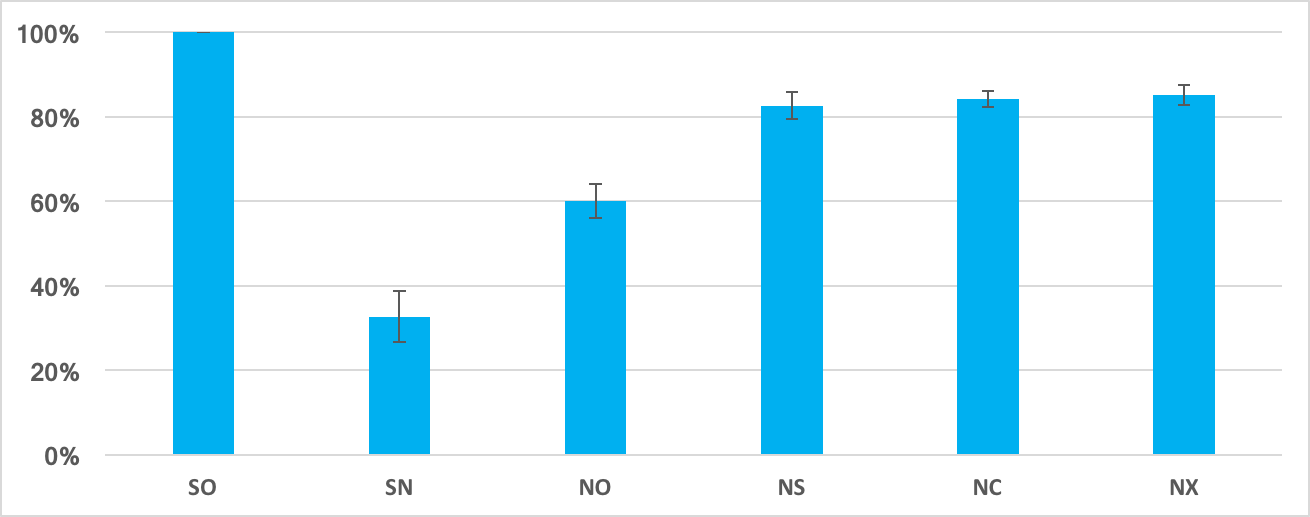
\includegraphics[max width=\textwidth]{experiment-1-results-chart}
	\caption{A comparison of the mean accuracy and 95\% confidence intervals of the models developed by the five methods.}
	\label{fig:experiment-1-results-chart}
\end{figure}

Table \ref{tab:experiment-1-results-table} and Figure \ref{fig:experiment-1-results-chart} compare the scores obtained from evaluating the models after training using the five methods. Training with symbols only (SO) produces the best model given the clear and consistent symbolic images. Training with the noisy handwritten digits only (NO) produces the worst model given the limited number of examples in the dataset. The three methods (NS, NC, NX) that developed models using noisy handwritten images as well as symbolic information show significant improvement over noisy only training. The results also show that there are no significant differences between the two methods of supplying symbols to the networks. However, the models that were trained using intermediate classification (NC and NX) have a smaller standard deviation.

\subsubsection{Discussion}

The experiments show that training a model with symbols results in a significant increase in the network accuracy over the models trained without the presence of symbols. The NC method that developed models to classify the operands as well as compute the addition did particularly well without the need for any additional inputs. The model does not accept a symbolic channel. Instead, by providing proper classification of the input operands while training, the model can be said to develop an implicit symbolic representation of the operands in the LSTM's recurrent context and transfer them from one step to the next.

The results presented in Table \ref{tab:experiment-1-results-table} and Figure \ref{fig:experiment-1-results-chart} show that there is no significant difference in the accuracy of the models trained using implicit symbols (NC) over the models trained with explicit symbols (NS). However, the experiment shows that the implicit symbol (NC) technique provides symbols to the network with the lowest predictive variance and therefore, we will use the implicit symbol technique in subsequent experiments.

Table \ref{tab:experiment-1-results-table} and Figure \ref{fig:experiment-1-results-chart} also show the results of testing the symbols only model (SO) using noisy data (SN). It is clear from the results that the network performs poorly. The model is not able to correctly map from the noisy handwritten digits to the classification labels and therefore is not able to successfully perform the addition.

\subsection{Experiment 2: Expanding Experiment 1 to use all four arithmetic operations} \label{sec:experiment-2}

\subsubsection{Objective}

The goal of this experiment is similar to Experiment 1 where we attempted to verify that the presence of symbols while training an artificial neural network results in significant increases in the network accuracy. Experiment 1 used only the addition operation. This experiment expands the dataset used to include all four arithmetic operations.

\subsubsection{Method}

For this experiment we use the \textbf{Noisy Inputs with Intermediate Classification (NC)} from the previous experiment as the model that is trained in the presence of symbols. Figure \ref{fig:sequential-model-symbols-noisy-times} depicts the NC model learning to do multiplication. \textbf{The Noisy Inputs Only (NO)} model is also used for comparison as the model trained without symbols. NO is slightly modified to provide output on its intermediate time steps. The output provided during training for these intermediate time steps is a vector with all its features set to a dummy value of 0.5 to signify that no symbol is provided. Figure \ref{fig:sequential-model-noisy-only-divide} shows an example of the NO model performing division.

The dataset used for Experiment 1 is expanded to include four different arithmetic operations (addition, subtraction, multiplication and division). For each operation, single digit inputs from the range of 0 to 9 are used to form combinations of operands and for each combination, ten MNIST examples are sampled. For both addition and multiplication, all 100 combinations are included in the dataset. However, for subtraction and division the combinations are selected so that for subtraction, no combinations that would result in negative outputs would be included and for division, division by zero is avoided. K-fold cross-validation is used, with k set to 5, to split the samples of each combination into a training, validation and test set. The training and testing of each model is repeated five times and the accuracy obtained on the test set is recorded for each attempt. Just like in Experiment 1, all combinations of digits are provided for training.

\begin{figure}[t]
	\centering
	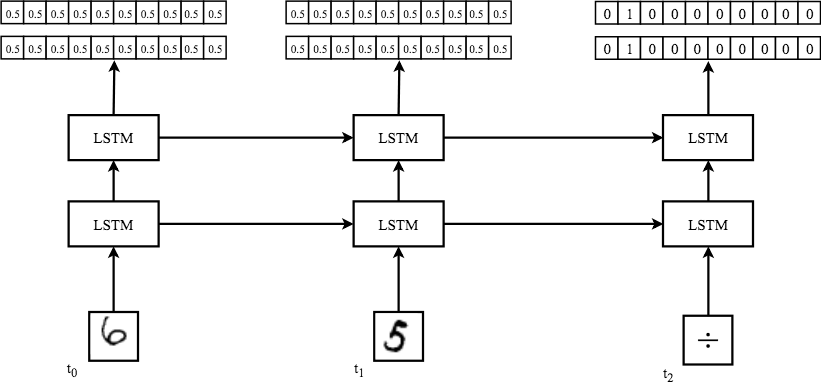
\includegraphics[max width=\textwidth]{sequential-model-noisy-only-divide}
	\caption{The Noisy Inputs Only (NO). A deep LSTM network that accepts a sequence of two operands and an operator modeling the operation: 6 / 5. Only noisy operands are provided. The output represents the quotient and the remainder, which are both 1.}
	\label{fig:sequential-model-noisy-only-divide}
\end{figure}

Both models have the same architectures used in Experiment 1. The models accept a sequence of three 28x28 images. The first two images are of the handwritten digits representing the operands of the operation. The third image is that of the operator. The models output two one-hot vectors representing the least and most significant values of the output at each time step. When each of the operands is presented, the network attempts to output the correct signals on the one-hot vector outputs representing the value of the digit presented on the input. When finally the operator is presented, the network is trained to perform the operation and output the result. Both models use two hidden LSTM layers each with 512 units.

\begin{figure}[t]
	\centering
	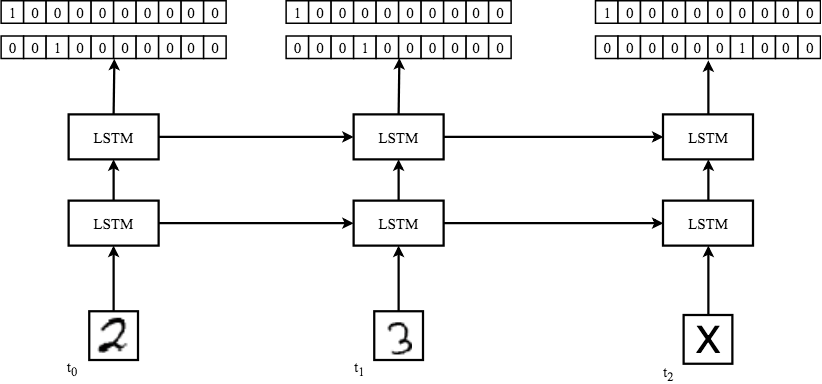
\includegraphics[max width=\textwidth]{sequential-model-symbols-noisy-times}
	\caption{Noisy Inputs with Intermediate Classification (NC). A deep LSTM network that accepts a sequence of two operands and an operator modeling the operation 2 x 3. Both the noisy operands and their corresponding symbolic information are provided alongside one another.}
	\label{fig:sequential-model-symbols-noisy-times}
\end{figure}

\subsubsection{Results}

\begin{table}[p]
	\center
	\caption{A comparison of the mean accuracy and standard deviation of the models trained with and without classification on all four arithmetic operations. Also shown is the p-value of a hypothesis t-Test when compared to the NO method.}
	\label{tab:experiment-2-results-table}
	\begin{tabular}{ |c|c|c|c| } 
		\hline
		Method & Accuracy (\%) & Standard Deviation  & p-value, t-Test with NO Method\\ 
		NO & 60.75 & 0.02 & NA \\  
		NC & 77.36 & 0.03 & 0.00092\\  
		\hline
	\end{tabular}
\end{table}

\begin{figure}[p]
	\centering
	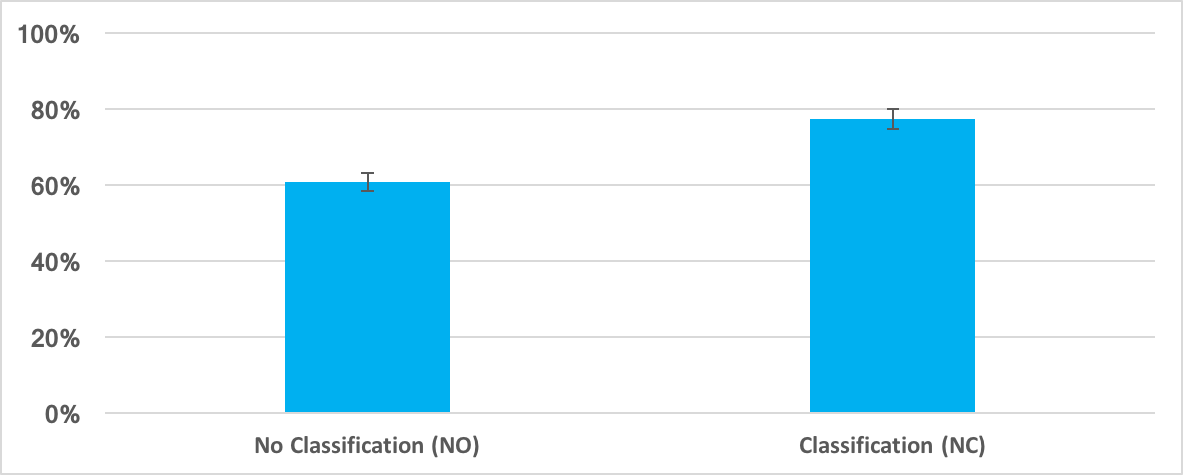
\includegraphics[max width=\textwidth]{experiment-2-results-chart}
	\caption{A comparison of the mean accuracy and 95\% confidence intervals of the models trained with and without classification on all four arithmetic operations.}
	\label{fig:experiment-2-results-chart}
\end{figure}

\begin{table}
	\center
	\caption{The mean accuracies of each arithmetic operation when tested on both the NO and NC models.}
	\label{tab:experiment-2-operations-table}
	\begin{tabular}{ |c|c|c|c|c| } 
		\hline
		Method & Addition (\%) & Subtraction (\%)  & Multiplication (\%) & Division (\%)\\ 
		NO & 63.35 & 60.77 & 61.4 & 57.48\\  
		NC & 78.5 & 77.71 & 80.23 & 73.0\\  
		\hline
	\end{tabular}
\end{table}

\begin{figure}[t]
	\centering
	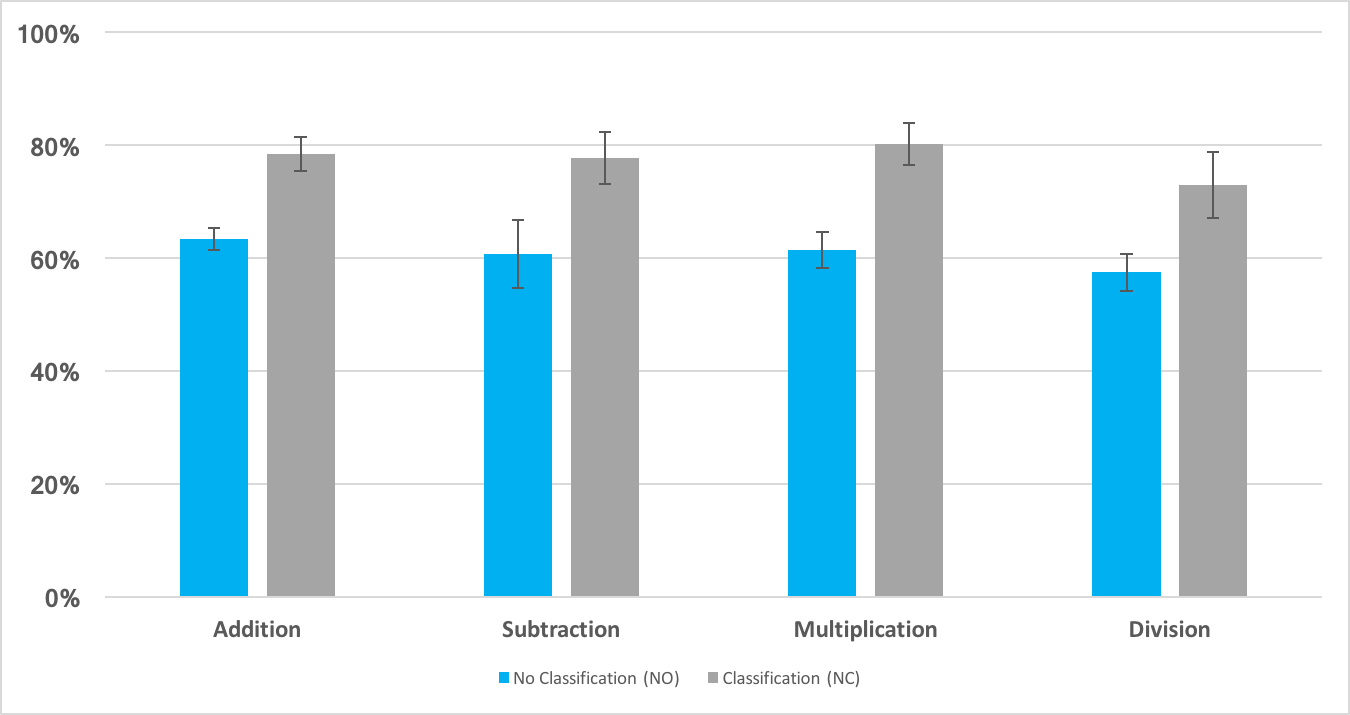
\includegraphics[max width=\textwidth]{experiment-2-operations-chart}
	\caption{A comparison of the mean accuracy and 95\% confidence intervals of each arithmetic operation on both models trained with and without classification.}
	\label{fig:experiment-2-operations-chart}
\end{figure}

Table \ref{tab:experiment-2-results-table} and Figure \ref{fig:experiment-2-results-chart} compare the results of the model trained without symbols (NO) with the model trained with symbols (NC). The model trained in the presence of symbols performs significantly better than the one trained without symbols. Table \ref{tab:experiment-2-operations-table} and Figure \ref{fig:experiment-2-operations-chart} show the accuracies obtained using each of these models when tested on each arithmetic operator independently.

\subsubsection{Discussion}

This experiment shows that the LSTM recurrent neural networks are capable of learning various types of arithmetic operations on images of handwritten digits and that the presence of symbolic knowledge during training significantly improves the accuracy of these models. With the exception of division, Table \ref{tab:experiment-2-operations-table} and Figure \ref{fig:experiment-2-operations-chart} show that when analyzing the accuracies of the models on each operator independently, we see that the mean accuracies are close to one another and close to the overall mean accuracy of the models. Division is a more complicated operation that involves finding a quotient and a remainder which could account of the reduced performance.

\subsection{Experiment 3: Comparing the Effect of Varying the Presence of Symbols on the Accuracy of Training} \label{sec:experiment-3}

\subsubsection{Objective}

In the previous experiments, we showed that the presence of symbols improves the effectiveness of recurrent neural networks in learning to perform arithmetic on images of handwritten digits when training using an impoverished dataset. In Section \ref{sec:theory-hypothesis-multi-task-learning} we proposed that this would be the expected behavior due to the beneficial effect of multi-task learning on all tasks being learned by the recurrent networks. In this experiment we attempt to further demonstrate this benefit.
 
Our goal is to show the relationship between the accuracy of the model in classifying the inputs on the intermediate time steps and the accuracy of the same model in producing the correct output for the given mathematical operation. The existence of this relationship should indicate that by correctly classifying the digits, the recurrent neural network is able to create internal features on the first two time steps that are then used on the third time step to perform the arithmetic operation. In the absence of these clear features, the network would rely only on the noisy handwritten inputs.

Besides establishing the relationship between the classification accuracy and the mathematical accuracy of our models, we also to vary the percentage of symbols included with each training example. The expected outcome here is that the higher the percentage of symbols present, the more accurate the classification accuracy will be and in turn the higher the accuracy of performing the arithmetic operation.

\subsubsection{Method}

The architectures constructed for this experiment are the same as the ones used in the previous two experiments. The models accept a sequence of three 28x28 images. The first two images are of the handwritten digits representing the operands of the operation. The third image is that of the operator. The networks output two one-hot vectors. When each of the operands are presented, the model attempts to output a one-hot encoded vector of the value of the operand. When the operator is presented, the network learns to compute and present the output. Two hidden layers are used each containing 512 LSTM units. All four arithmetic operations are used together during training.

The dataset used in Experiment 2 in Section \ref{sec:experiment-2} is replicated into five sets, with some modifications, for use in this experiment. Each combination now includes eight MNIST samples instead of ten, where four are used for training, two for validation and two for testing. This makes the process of varying symbols easier. Each of the five replicas are modified to vary the number of symbols included with each digit combination during training. The first set has no symbols, meaning a vector with all features set to 0.5 is provided as a dummy output for the intermediate classification time steps. The second dataset has 25\% of the MNIST samples in each combination include a symbol whereas the rest use the 0.5 dummy values. The 25\% symbols are distributed such that, out of the four training samples, one has a symbol and the rest do not. The third dataset has 50\% symbols meaning that out of the four training examples per combination two include their corresponding symbols. The fourth dataset has 75\% of the training examples include symbols, meaning three out of four examples per combination include their corresponding symbol. Finally, the fifth dataset, the 100\% symbols dataset, includes symbols for all examples.

Five models were trained each using one of the datasets described above. The networks were trained using the Adam optimizer with the mean square error as the loss function and a learning rate of 0.001. Training is performed over 200 epochs in batches of 100 and the model performing best on the validation set is saved. Each model is trained five times using 5-fold cross-validation where all digit combinations are used. Instead of recording the accuracy of each model as was done in the previous experiments, here we split the accuracy into four new metrics. They are as follows:
\begin{itemize}
	\item False Classification/False Operation \textbf{(FC/FO)}: The percentage of test samples that classify incorrectly during the intermediate time steps that also produce incorrect outputs for the mathematical operation.
	\item False Classification/True Operation \textbf{(FC/TO)}: The percentage of test samples that classify incorrectly during the intermediate time steps that produce correct outputs for the operation.
	\item True Classification/False Operation \textbf{(TC/FO)}: The percentage of test samples that classify correctly during the intermediate time steps that produce incorrect outputs for the operation.
	\item True Classification/True Operation \textbf{(TC/TO)}: The percentage of test samples that classify correctly during the intermediate time steps that also produce correct outputs for the operation.
\end{itemize}

The epoch number that results in the most optimum set of weights for each percentage of symbols used is also recorded, to understand the effect of symbols on the efficiency of training with and without symbols.

\subsubsection{Results}

\begin{table}[p]
	\center
	\caption{A comparison of the mean FC/FO percentage, standard deviation and the p-value of a hypothesis t-Test when compared to the 0\% symbols model.}
	\label{tab:experiment-3-results-table-fcfo}
	\begin{tabular}{ |c|c|c|c| } 
		\hline
		\% Symbols Present & FC/FO (\%) & Standard Deviation  & p-value\\ 
		0\% & 55.8 & 0.063 & NA \\  
		25\% & 39.80 & 0.03 & 0.00493\\  
		50\% & 26.20 & 0.042 & 0.00141 \\  
		75\% & 17.05 & 0.023 & 0.00033\\  
		100\% & 13.60 & 0.012 & 0.00016\\  
		\hline
	\end{tabular}
\end{table}

\begin{table}[p]
	\center
	\caption{A comparison of the mean FC/TO percentage, standard deviation and the p-value of a hypothesis t-Test when compared to the 0\% symbols model.}
	\label{tab:experiment-3-results-table-fcto}
	\begin{tabular}{ |c|c|c|c| } 
		\hline
		\% Symbols Present & FC/TO (\%) & Standard Deviation  & p-value\\ 
		0\% & 37.55 & 0.0672 & NA \\  
		25\% & 27.95 & 0.0387 & 0.0031\\  
		50\% & 11.50 & 0.0351 & 0.00141 \\  
		75\% & 5.40 & 0.0137 & 0.00084\\  
		100\% & 2.45 & 0.0042 & 0.00016\\  
		\hline
	\end{tabular}
\end{table}

\begin{table}[p]
	\center
	\caption{A comparison of the mean TC/FO percentage, standard deviation and the p-value of a hypothesis t-Test when compared to the 0\% symbols model.}
	\label{tab:experiment-3-results-table-tcfo}
	\begin{tabular}{ |c|c|c|c| } 
		\hline
		\% Symbols Present & TC/FO (\%) & Standard Deviation  & p-value\\ 
		0\% & 3.70 & 0.0106 & NA \\  
		25\% & 15.05 & 0.0214 & 0.00183\\  
		50\% & 23.20 & 0.01024 & 0.02209 \\  
		75\% & 13.55 & 0.0107 & 0.00013\\  
		100\% & 8.15 & 0.0158 & 0.01742\\  
		\hline
	\end{tabular}
\end{table}

\begin{table}[p]
	\center
	\caption{A comparison of the mean TC/TO percentage, standard deviation and the p-value of a hypothesis t-Test when compared to the 0\% symbols model.}
	\label{tab:experiment-3-results-table-tcto}
	\begin{tabular}{ |c|c|c|c| } 
		\hline
		\% Symbols Present & TC/TO (\%) & Standard Deviation  & p-value\\ 
		0\% & 2.95 & 0.0166 & NA \\  
		25\% & 17.20 & 0.0148 & 0.00043\\  
		50\% & 39.10 & 0.0853 & 0.00179 \\  
		75\% & 64.00 & 0.0301 & 0.0\\  
		100\% & 75.80 & 0.0213 & 0.0\\  
		\hline
	\end{tabular}
\end{table}

\begin{figure}[p]%
	\centering
	\subfloat[False Classification/False Operation]{{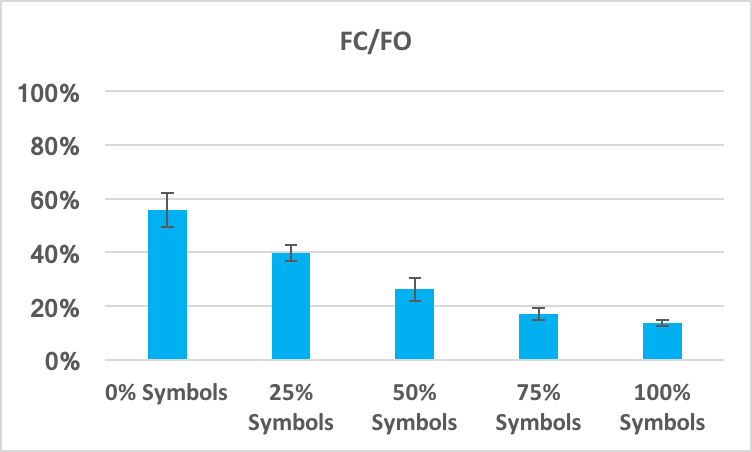
\includegraphics[width=0.5\textwidth]{experiment-3-results-chart-fc-fo} }}\label{fig:experiment-3-results-chart-fc-fo}%
	\subfloat[False Classification/True Operation]{{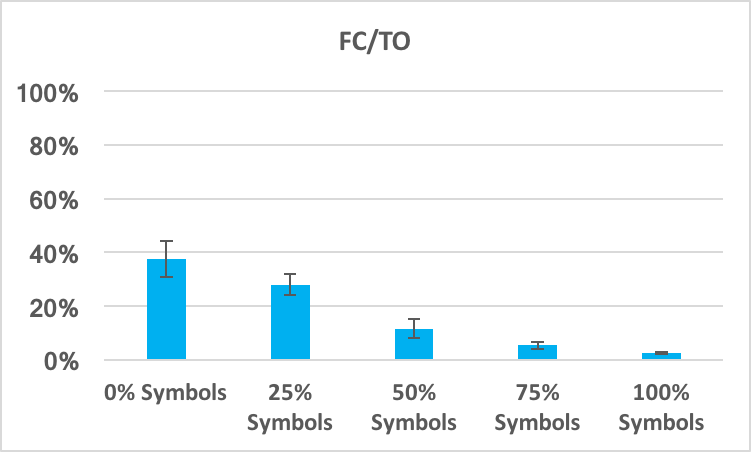
\includegraphics[width=0.5\textwidth]{experiment-3-results-chart-fc-to} }}\label{fig:experiment-3-results-chart-fc-to}%
	
	\subfloat[True Classification/False Operation]{{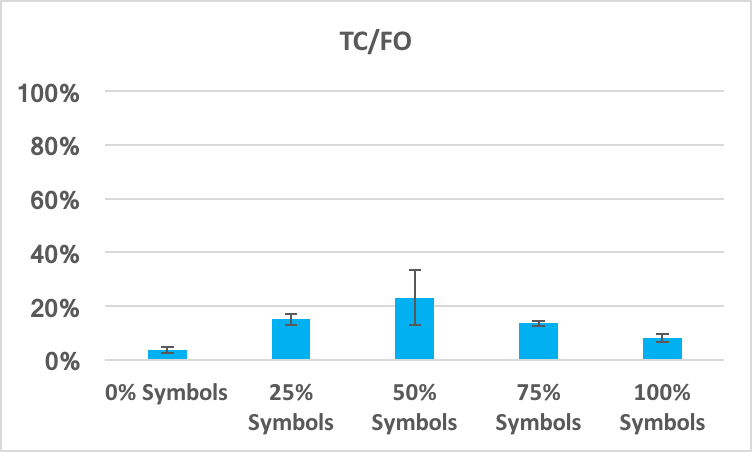
\includegraphics[width=0.5\textwidth]{experiment-3-results-chart-tc-fo} }}\label{fig:experiment-3-results-chart-tc-fo}%
	\subfloat[True Classification/True Operation]{{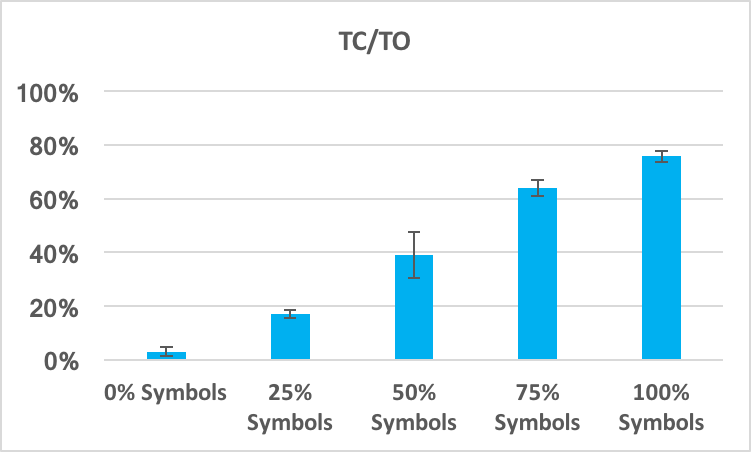
\includegraphics[width=0.5\textwidth]{experiment-3-results-chart-tc-to} }}\label{fig:experiment-3-results-chart-tc-to}%
	\caption{A comparison of the four metrics FC/FO, FC/TO, TC/FO, TC/TO along with their corresponding 95\% confidence intervals for each of the five models developed.}%
	\label{fig:experiment-3-results-chart}%
\end{figure}

Tables \ref{tab:experiment-3-results-table-fcfo} to \ref{tab:experiment-3-results-table-tcto} present the mean FC/FO, FC/TO, TC/FO, TC/TO accuracies for each of the datasets used along with the standard deviations and the p-test score of a hypothesis t-Test compared to the 0\% model. Figure \ref{fig:experiment-3-results-chart} shows the same results presented in graphical form. Table \ref{tab:experiment-3-results-epochs} presents the number of epochs needed for the network to discover the optimum set of weights for each of the five datasets.

\begin{table}[h]
	\center
	\caption{A comparison of the average epoch number at which the optimum weights were discovered for each of the models trained.}
	\label{tab:experiment-3-results-epochs}
	\begin{tabular}{ |c|c| } 
		\hline
		\% Symbols Present & Mean Epoch Number\\ 
		0\% Symbols & 4.2\\  
		25\% Symbols & 10.0\\  
		50\% Symbols & 11.0\\  
		75\% Symbols & 15.8\\  
		100\% Symbols & 38.0\\  
		\hline
	\end{tabular}
\end{table}

\subsubsection{Discussion}

It is clear from Table \ref{tab:experiment-3-results-table-tcto} and Figure \ref{fig:experiment-3-results-chart}(d) that more training examples with symbolic classification data improves the correct output of the operations (TO), particularly when the classification is also correct (TC) (75.8\% of the time with 100\% symbols), and rarely, as shown in Table \ref{tab:experiment-3-results-table-fcto} and Figure \ref{fig:experiment-3-results-chart}(b) when the classification is incorrect (FC) (only 2.45\% of the time with 100\% symbols).

Inversely, as shown in Table \ref{tab:experiment-3-results-table-fcfo} and Figure \ref{fig:experiment-3-results-chart}(a), incorrect output (FO) for a mathematical operator occurs frequently with false classification (FC) (13.6\% of the time with 100\% symbols). It also makes sense that as the percentage of false classifications (FC) declines (due to more symbols in the training set) the percentage of false operation (FO) outputs also declines, because the probability of an operation being performed on the wrong operands decreases.

These results show that the presence of symbols improves the accuracy of classification which in turn improves the accuracy of performing the operation. Classifying the handwritten operands creates an internal representation of the digits that is retained by the LSTM recurrent connections. In the presence of symbols, this representation is learned more consistently for each digit, reducing the variations of the handwritten digits and therefore improving the model's accuracy when performing the operation. This is a recurrent multi-task learning effect that provides beneficial results.

The TC/FO graph of Figure \ref{fig:experiment-3-results-chart}(c) on the other hand says that incorrect operation output (FO) occurs most frequently (23.2\% of the time) when 50\% of the training examples have classification signals and the test examples operands are classified correctly (TC). In fact, the percentage of FO examples is almost as high for TC/FO at 50\%, 75\% and 100\% as they are for FC/FO. This makes it clear that there are limits to the system's ability to get correct operation outputs (TO) even when it has TC for certain examples.

\begin{figure}[t]
	\centering
	
\includegraphics[max width=\textwidth]{tc-fo-example}
	\caption{Example of a TC/FO operation. The operation 5 + 4 is classified correctly, however the output is still false.}
	\label{fig:tc-fo-example}
\end{figure}

This limitation can be due to the fact that the noisy handwritten digits still retain some influence over the network that forces the model to use the noisy inputs for pattern matching instead of the clearer internal representations. Figure \ref{fig:tc-fo-example} shows an example of one of the TC/FO cases trained with 50\% symbols. The handwritten digits are shown along with the result of classification and the result of the operation. The operation is that of 5 + 4. The handwritten digits are classified correctly, however the output of 5 is incorrect. This example shows that the model was still being influenced by the confusing handwritten digits. It might have confused the first operand 5 for the digit 1.

Looking at the results in Table \ref{tab:experiment-3-results-epochs} we see that the more symbols are used the longer it takes for the network to converge onto an optimum decision function. We initially predicted that providing clearer symbols would make the learning process more efficient, but that apparently is not the case. We now understand that without the symbolic information, the gradient descent algorithm will converge to a local minimum early in the training process resulting in the poor classification results and therefore less accurate mathematical operation output. The introduction of more symbols forces the gradient descent algorithm to search longer for an appropriate representation in weight space that is compatible with both the symbol classification and the mathematical operation output.


\section{Explaining the Role of Symbols} \label{sec:empirical-studies-explaining-the-role-of-symbols}

In the previous set of experiments we showed that our theory holds given that the models trained with the aid of symbols outperformed the models that were trained in the absence of symbols. We also showed that there was not much difference in the effectiveness of both the explicit and implicit forms of providing symbols. The next set of experiments investigate the second objective of our research which is to establish the reason why symbols improve learning in artificial neural networks. We start with an experiment that attempts to show that symbols help the artificial learner discover a general solution to the problem, similar to how they are used by humans. Based on the results, we explain the role that symbols play in the learning process.

\subsection{Experiment 4: Recurrent Neural Network's Ability to Discover an Algorithm for Arithmetic Operations} \label{sec:experiment-4}

\subsubsection{Objective}

In Section \ref{sec:theory-approach-methodology-pattern-matching-vs-learning-an-algorithm} we described two possible methods a neural network can learn to perform these arithmetic operations, either by (1) memorizing the input patterns along with the corresponding output, effectively doing pattern matching, or (2) by learning an algorithm that is able to generalize to patterns that the model has not seen before. In the prior experiments, we have shown the former to be true. However, we wish to show that with the aid of appropriate symbols a recurrent neural network is capable of discovering a representation of an algorithm that performs the corresponding mathematical operation.

In this experiment, we attempt to understand whether or not recurrent neural networks are able to accomplish that goal. To verify if that is indeed the case, we train our models on a subset of the combinations of digits. The remaining set of combinations are used to test the trained models. If the models perform well on this unseen set of combinations, this would show that the recurrent neural networks are able to generalize to unseen combinations of digits and is therefore proof that the machine learning system has discovered an algorithm for the arithmetic operations. Otherwise the models trained in the previous experiments are simply doing pattern matching.

\subsubsection{Method}

We develop and train five models for this experiment to perform all four arithmetic operations on the MNIST dataset of handwritten digits. Similar to how the models in Experiment 3 in Section \ref{sec:experiment-3} were trained,  the first model is trained with 0\% symbols, the second with 25\% symbols present, the third with 50\% symbols present, the fourth with 75\% symbols present and finally the fifth with 100\% symbols. All five models have the same architecture that accepts a sequence of three 28x28 images. The first two images are of the handwritten digits representing the operands of the operation. The third image is that of the operator. The models output two one-hot vectors. For the first two time steps the output is the one-hot vector representation of the input digits. On the third step the output is a one-hot vector representation of the result of the operation. Two hidden layers are used each with 512 LSTM units.

The five datasets used in Experiment 3 are also used for this experiment. The difference is that not all combinations of digits are used for training. For each of the five datasets, a subset composed of 80\% of the digit combinations are selected for training for each of the four operators, making sure that each unique digit would be present at least once on either side of the arithmetic operator. We call this the ``seen" dataset since the models are exposed to these combinations during training. The remaining 20\% combinations are the ``unseen" test set that we use to determine if the models are able to generalize to unseen operations and therefore are able to learn an algorithm. The samples in the seen training set are distributed into training, validation and test sets using k-fold cross-validation where k is set to 5. All the samples in the unseen test set are used for testing after the models are trained on the seen dataset. The networks are trained using the Adam optimizer with the mean square error as the loss function and a learning rate of 0.001. Training is performed over 200 epochs in batches of 100 and the model performing best on the validation set is saved and used for testing.

\subsubsection{Results}

\begin{table}[p!]
	\center
	\caption{A comparison of the mean accuracy and standard deviation along with the p-value of a hypothesis t-Test when compared to the 0\% symbols model when tested on the test set of \textbf{seen} combinations.}
	\label{tab:experiment-4-results-table-seen}
	\begin{tabular}{ |c|c|c|c| } 
		\hline
		\% Symbols Present & Accuracy (\%) & Standard Deviation  & p-value\\ 
		0\% & 40.68 & 0.0420 & NA \\  
		25\% & 57.48 & 0.0211 & 0.00383\\  
		50\% & 61.38 & 0.0504 & 0.0 \\  
		75\% & 69.44 & 0.0136 & 0.0\\  
		100\% & 78.23 & 0.0134 & 0.0\\  
		\hline
	\end{tabular}
\end{table}

\begin{table}[p!]
	\center
	\caption{A comparison of the mean accuracy and standard deviation along with the p-value of a hypothesis t-Test when compared to the 0\% symbols model when tested on the test set of \textbf{unseen} combinations.}
	\label{tab:experiment-4-results-table-unseen}
	\begin{tabular}{ |c|c|c|c| } 
		\hline
		\% Symbol Presence & Accuracy (\%) & Standard Deviation  & p-value\\ 
		0\% & 1.00 & 0.0 & NA \\  
		25\% & 3.00 & 0.0240 & 0.374\\  
		50\% & 4.00 & 0.0367 & 0.208 \\  
		75\% & 2.00 & 0.0240 & 0.621\\  
		100\% & 3.00 & 0.0392 & 0.477\\  
		\hline
	\end{tabular}
\end{table}

\begin{figure}[p!]%
	\centering
	\subfloat[Seen Test Combinations]{{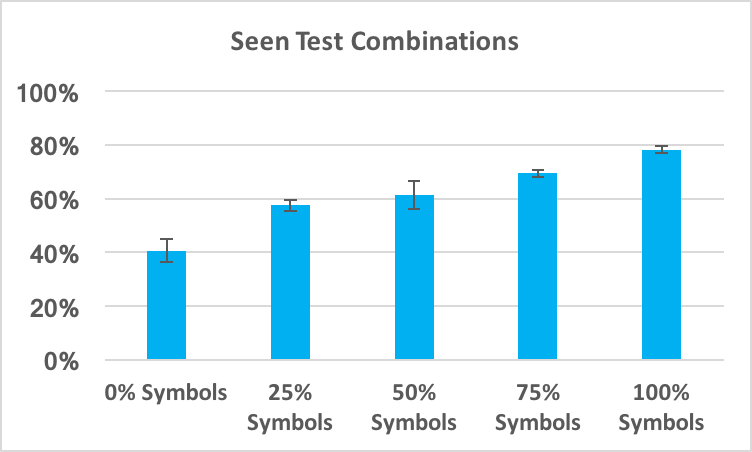
\includegraphics[width=0.5\textwidth]{experiment-4-results-chart-seen}}}%
	\subfloat[Unseen Test Combinations]{{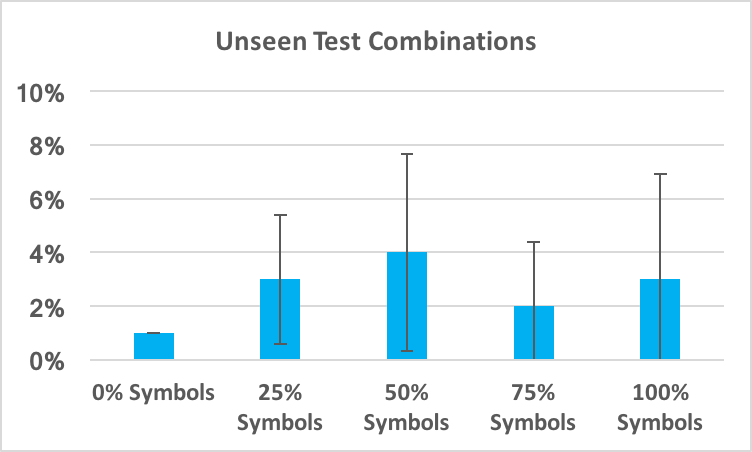
\includegraphics[width=0.5\textwidth]{experiment-4-results-chart-unseen}}}%
	\caption{A comparison of the mean accuracy and 95\% confidence intervals for each of the models when tested on both the \textbf{seen} and \textbf{unseen} test combinations.}
	\label{fig:experiment-4-results-chart}
\end{figure}

Table \ref{tab:experiment-4-results-table-seen} shows the mean accuracy, standard deviation and t-test p-value scores for the test set which uses the same operand combinations that the models were trained on. Table \ref{tab:experiment-4-results-table-unseen} shows these same metrics when the same models are tested on operand combinations they have never seen before. Figure \ref{fig:experiment-4-results-chart} shows graphs of these results along with 95\% confidence intervals.

Table \ref{tab:experiment-4-results-table-seen} shows similar accuracies to those obtained in Experiment 2 with the models trained in the presence of symbols outperforming the ones trained without symbols. However, the models when tested on the unseen dataset show poor performance regardless of whether they are trained with symbols or not.

\subsubsection{Discussion}

It is clear from these results that the current recurrent neural network models are unable to generalize to unseen combinations of operands. They are unable to discover a representation for an algorithm for the arithmetic operations. The models perform well on the previously experienced combinations by developing a sequential mapping function for those seen operand combinations.

In the next section, we describe an experiment that examines our theory in Section \ref{sec:theory-approach-methodology-pattern-matching-vs-learning-an-algorithm} to understand how this pattern matching works and how the presence of symbols makes this process more effective. Later, we present a different approach that uses a modified representation of the symbols as discussed in Section \ref{sec:theory-approach-methodology-temperature-encoding}. Using this new representation, we are able to develop a model that performs well on unseen test sets.

\subsection{Experiment 5: Using Symbols Only to Learn Arithmetic Operations} \label{sec:experiment-5}

\subsubsection{Objective}

We have shown that the presence of symbols improves the accuracy of learning with a limited dataset of noisy examples. In Experiment 3 in Section \ref{sec:experiment-3}, we showed that this was due to the effectiveness of symbols at learning a mapping function. In the previous experiment however, we have failed to show that symbols allow neural networks to go beyond learning mapping functions and actually discover an algorithm to perform the arithmetic operations. In this experiment, we constrain and simplify the problem to make it easier for the models we are developing to reach the desired objective of learning an algorithm. We will train recurrent neural networks to perform addition using the symbolic features alone without introducing the MNIST handwritten digits. The goal here is the same as that of Experiment 4 in Section \ref{sec:experiment-4} where we want to force the network to generalize to unseen combinations of digits.

Besides constraining the input features, we also take a different approach to analyzing the behavior of the trained recurrent neural networks, by visualizing the outputs of the hidden layers of the models using a concept know as activations clustering. With activations clustering, the output value of each unit in the hidden recurrent layers ($h_t$) is mapped to a pixel intensity where an output of -1 would map to 0 and an output of 1 would map to 255. Each unit would be assigned a region on an image and that region would be filled using the pixel intensity assigned when a digit is presented to the trained model on each time step. Figure \ref{fig:activations-cluster-explained} shows an example of an activations cluster. The activations clusters should allow us to confirm that the presence of symbols allows for more consistency in the representation which leads to the improved accuracy. The clusters may also shed some insight into why the networks fail to develop an algorithm.

We will also add an additional time step to the recurrent sequence. Like before, the first time step is the right hand operand, the second time step is the left hand operand, the third time step is the operator which now only outputs the least significant digit of the result. The additional fourth time step is an equals sign which signifies to the model to output the most significant digit of the result. This change was made so that we can determine if there is any relationship between what is being output on the least significant one-hot vector and the most significant one. This also resembles how we as humans do addition. We consume one input digit at a time and we produce one output digit at a time, making note of carry forward digits, if necessary.


\subsubsection{Method}

\begin{figure}
	\centering
	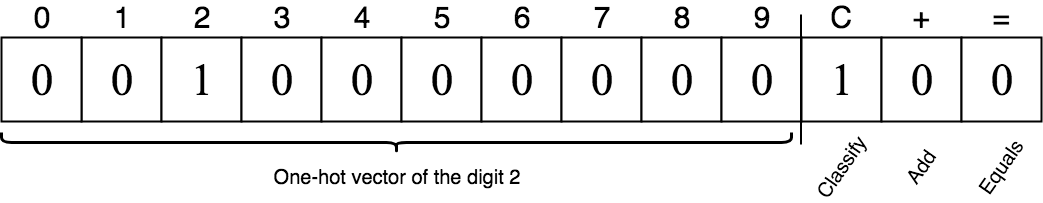
\includegraphics[max width=\textwidth]{experiment-5-input}
	\caption{An example of an input vector for the digit 2 on the first time step. The first ten features are for the one-hot symbol. The 11th (C) feature when set, feature instructs the RNN to output the class at that time step. The 12th (+) feature when set, instructs the network to output the least significant digit of the result. The 13th (=) feature when set, instructs the RNN to output the most significant digit of the result.}
	\label{fig:experiment-5-input}
\end{figure}

The models developed for this experiment accept a sequence of four vectors, each vector is composed of thirteen elements. Figure \ref{fig:experiment-5-input} depicts the structure of the input vectors. The first ten elements represent the one-hot vector. Element 11 is set to one when we want the network to perform classification and output a one-hot vector representing the input operand, zero otherwise. This is always set to one when the operands are presented to the network to signify to the network that an input symbol is being presented on the intermediate time steps. Element 12 is set to one at the third time step. This element indicates that the addition should be performed and that the least significant digit of the output should be produced. The element is set to zero otherwise. Finally, element 13 is set to one on the fourth time step when the most significant digit of the result of the addition is presented on the output.

\begin{figure}
	\centering
	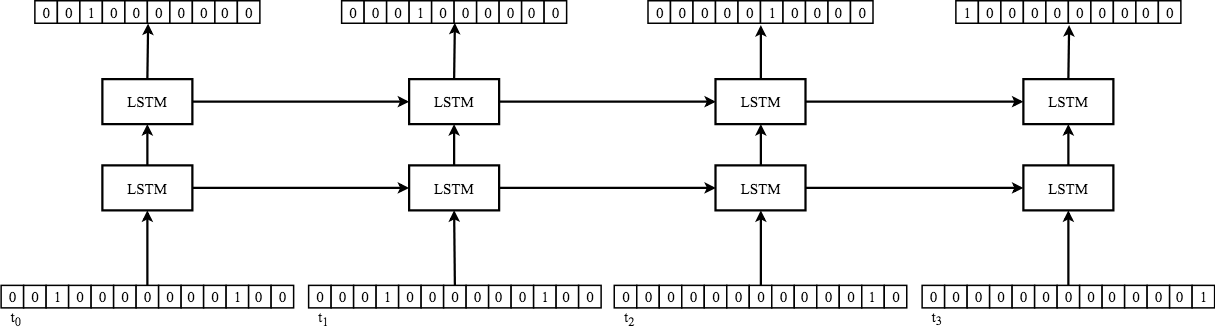
\includegraphics[max width=\textwidth]{experiment-6-architecture}
	\caption{The constrained symbol only architecture learning to perform 2 + 3.}
	\label{fig:experiment-6-architecture}
\end{figure}

The output layer of the models consists of 10 elements representing a one-hot vector output. When the first operand is presented on the input layer, the network outputs the same digit on the output layer. The same goes for the second operand on the second time step. When an input that has the 12th element set to one is presented on the third time step, the network outputs the least significant digit of the result of adding the operands together. Finally, on the fourth time step when an input having the 13th element set to one is presented to the model, the model outputs the most significant digit of the addition. Figure \ref{fig:experiment-6-architecture} depicts how the input and output layers interact on each time step.

A total of four recurrent neural network architectures were developed using the same input and output layer structures presented above. The models vary in the number and size of the recurrent hidden layers.  The following lists the composition of the hidden layers for each of the four models developed:
\begin{itemize}
	\item \textbf{Model A}: One hidden layer with 10 LSTM units each.
	\item \textbf{Model B}: Two hidden layers with 10 LSTM units each.
	\item \textbf{Model C}: Three hidden layers with 10 LSTM units each.
	\item \textbf{Model D}: Two hidden layers with 20 LSTM units each.
\end{itemize}

The dataset is composed by forming all possible 100 combinations of operands. A subset of 80 combinations are selected for training from that dataset, making sure that each unique digit would be present at least once on either side of the addition operator. That same training set is also used for validation and as the test set of seen combinations. The remaining 20 combinations are used as the unseen combinations test set. Each model is trained and tested five times and the mean accuracy of each model is recorded when applying both the seen test set and the unseen test set on the trained model. Training is performed over 5000 epochs in batches of 10 using the Adam optimizer algorithm and the mean square error loss function with a learning rate of 0.001.

\subsubsection{Results}

\begin{figure}
	\centering
	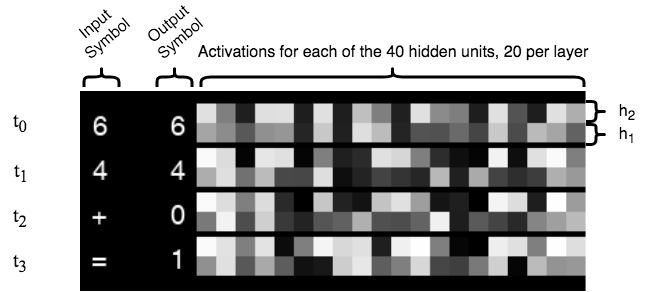
\includegraphics[max width=\textwidth]{activations-cluster-explained}
	\caption{An activations cluster generated when presenting the one-hot symbols of the operation 6 + 4 to the trained Model D. The symbols are displayed in this image as digits for clarity.}
	\label{fig:activations-cluster-explained}
\end{figure}

Table \ref{tab:experiment-6-results-table} shows the mean accuracies for each of the architectures developed. The table shows these values for both the full training set and the unseen test set. Figures \ref{fig:activations-cluster-explained} and \ref{fig:activations-cluster-carry} show some of the activations clusters that are produced when applying the seen dataset to Model D (the best performing model).

Figure \ref{fig:activations-cluster-explained} shows the result of rendering the activations cluster when applying the operand sequence of 6 + 4 to the trained Model D. The figure shows four rows of items, each row represents a single time step. For each time step, the figure depicts the input to the network, the output the network produces and the activations on the hidden units. The inputs and outputs are rendered in the figure as digits for clarity. Forty activations are shown for each time step, one for each hidden unit. The activations are split into two rows, each row holds the activations for one of the two hidden layers.

\begin{table}[h]
	\center
	\caption{A comparison of the mean accuracy of each of the four models developed when tested on the test set of \textbf{seen} combinations as well as the test set of \textbf{unseen} combinations.}
	\label{tab:experiment-6-results-table}
	\begin{tabular}{ |c|c|c| } 
		\hline
		Model & Accuracy - Seen (\%) & Accuracy - Unseen (\%)\\ 
		Model A & 75.0 & 5.0\\  
		Model B & 75.0 & 5.0\\  
		Model C & 75.0 & 5.0\\  
		Model D & 100.0 & 5.0\\
		\hline
	\end{tabular}
\end{table}

\subsubsection{Discussion}

It is clear from the results that even when constraining the model to only use one-hot symbols as inputs, the recurrent networks fail to generalize to the unseen dataset, even though they perform very well on the seen dataset. This shows that even when using clear one-hot symbols the neural network is still not able to discover a set of weights that can represent an algorithm that performs the addition operation.

\begin{figure}
	\centering
	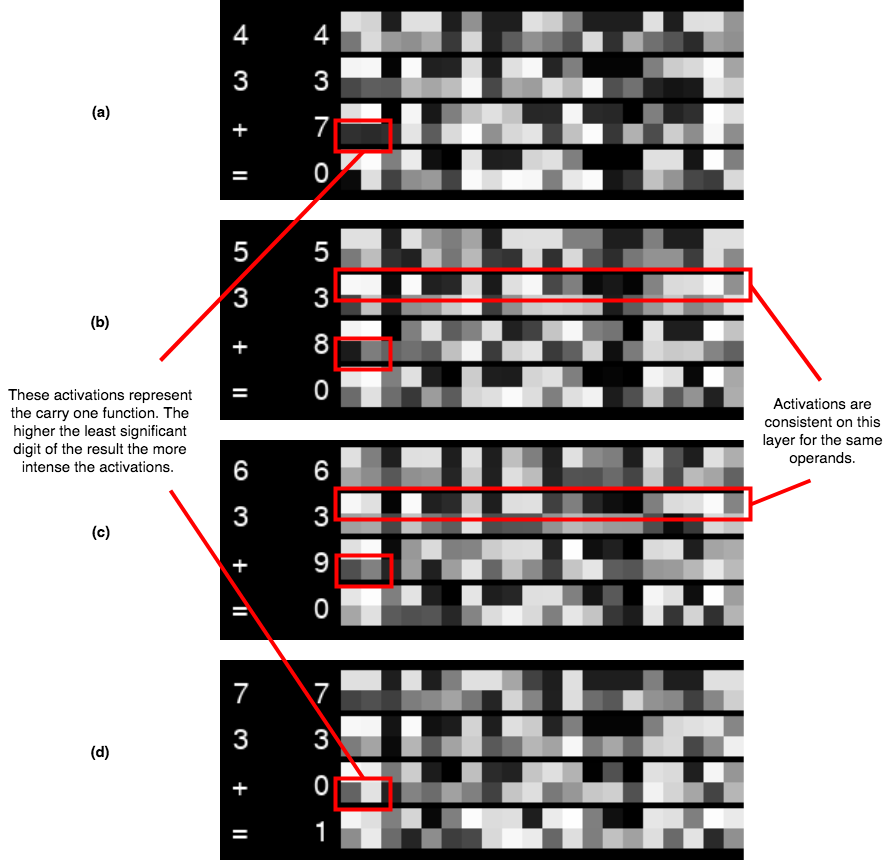
\includegraphics[max width=\textwidth]{activations-cluster-carry-annotated}
	\caption{A series of activations from Model D showing how the intensity in the bottom left region of the third time step changes when the output transitions from 7 through 8 and 9 to 10.}%
	\label{fig:activations-cluster-carry}%
\end{figure}

When analyzing the sequence of activations clusters in Figure \ref{fig:activations-cluster-carry}, we notice that the activations on the top layer ($h_2$) on any of the first two time steps are always consistent when the same operands are presented as exhibited by the digit 3 on the second time step of Figures \ref{fig:activations-cluster-carry} (a) to \ref{fig:activations-cluster-carry} (d). Also, the least and most significant digit outputs always have consistent activations on the top layer for the same results (see the fourth time step in Figures \ref{fig:activations-cluster-carry} (a), \ref{fig:activations-cluster-carry} (b) and \ref{fig:activations-cluster-carry} (c) and the third time step in Figure \ref{fig:activations-cluster-carry} (d)). By ``consistent" we mean that the same hidden units are producing the same intensities. These observations are in-line with the findings of Experiment 3 in Section \ref{sec:experiment-3} which shows that when successfully classifying the input digits, the recurrent neural networks discover a consistent internal representation that facilitates the execution of the arithmetic operations.

Another interesting pattern can be observed when analyzing the transition from the least significant digit time step to the most significant digit time step (see Figure \ref{fig:activations-cluster-carry}). The two most left-hand activations on the lower layer of the third (least significant digit) time step tend to be dark (indicating lower activations) when the least significant digit of the result is closer to zero than nine. The higher that digit the lighter the activations become. The variation in activations indicates that there is a signal being carried over from the least significant digit time step to the most significant digit time step. That signal forces the most significant output to flip from a zero to a one. When comparing this behavior with how we as humans perform addition, this process resembles the carry-one approach when writing out arithmetic problems with pen and paper. This shows that though for the most part the networks are still learning a mapping function, there are still some elements of an algorithm being developed within the network.

When further analyzing how humans learn to perform addition, we tend to convert the numbers into concepts that can be counted. More specifically with children, we represent numbers as collections of objects. So, 5 + 3 for example will be translated to a child as counting five ``apples" and counting another three ``apples" on top of the initial five. The symbols are able to represent quantity and ordinal relationships. One-hot vectors on the other hand don't capture these concepts; they are able to represent classes of digits which is why they assist in the development of good classifiers, but fail to develop models that can generally perform arithmetic. In the next set of experiments we use a different encoding for our symbols that better captures the ordinal nature of the digits.

\section{Temperature Encoding Experiments} \label{sec:empirical-studies-temperature-encoding-experiments}

So far we were able to show that symbols improve the effectiveness of the learning process when training neural networks on limited datasets. We have however failed to show that they can generalize to digit combinations that they have not seen before. In Section \ref{sec:theory-approach-methodology-temperature-encoding} we described an alternative representation for our symbols, namely the temperature encoded symbols. We explained our expectation that temperature encodings will improve the ability of the networks to generalize to unseen combinations since they are able to encapsulate three characteristics that are important in developing an algorithm that performs arithmetic. Specifically, these characteristics are, (1) the ability of the symbols to represent the ordinal relationship between digits, (2) the ability to represent the quantity of the digits and (3) the ability to capture the function of the operator. The prior experiment showed that one-hot vectors are capable of capturing the function of the operator, as shown by the ability of the models to internally represent the carry forward behavior of addition. They however fail in providing the other two properties. This final set of experiments investigates the ability of temperature encoded symbols to capture all three characteristics and presents a solution to our problem. 

\subsection{Experiment 6: Temperature Encoding} \label{sec:experiment-6}

\subsubsection{Objective}

When a symbol is represented as a temperature encoded vector, the symbol is represented as an array where a number of consecutive elements equal to the value of the digit being represented are set to one, the rest are set to zero. Figure \ref{fig:temperature-encoding} shows a depiction of a temperature encoded symbol of the number 5. We believe that symbols encoded using this representation can capture the quantitative and ordinal meaning of the digits and would therefore help the recurrent neural network learn an algorithm for arithmetic operations as opposed to simply learning a classifier or mapping function.

The goal of this experiment is to determine empirically whether or not models trained using the temperature encoded symbols have the ability to discover a decision function that can represent the algorithm that performs addition. We constrain the experiment to only use symbols as in Experiment 5. The models accept a sequence of operands encoded in the temperature encoding and outputs values encoded in the temperature encoding as well. The performance of the trained model is tested against both the training set as well as an unseen test set to determine if the model can generalize to unseen combinations of operands. 

\subsubsection{Method}

\begin{figure}
	\centering
	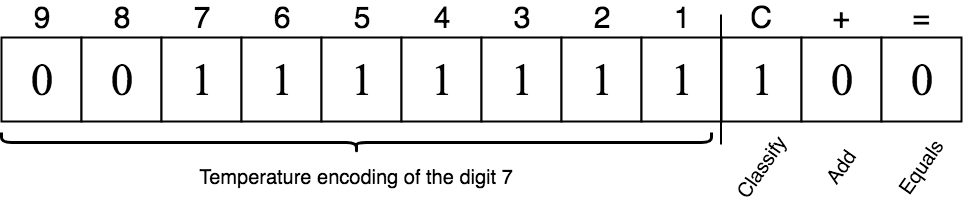
\includegraphics[max width=\textwidth]{experiment-6-input}
	\caption{An example of an input vector for the digit 7 on the first time step. The first nine features are for the temperature encoded symbol. The 10th (C) feature when set, instructs the RNN to output the class at that time step. The 11th (+) feature when set, instructs the network to output the least significant digit of the result. The 12th (=) feature when set, instructs the RNN to output the most significant digit of the result.}
	\label{fig:experiment-6-input}
\end{figure}

Three models are developed that learn to perform addition on temperature encoded symbols. Figure \ref{fig:sequential-model-temperature-symbols} shows an example of a recurrent neural network using temperature encoding to learn to do addition. The models accept a sequence of four vectors 12 elements each. Figure \ref{fig:experiment-6-input} depicts an example input. The first nine elements hold an operand represented as a symbol encoded using a temperature encoding. The 10th element indicates to the network to classify the input, meaning that if it is set to one, the model should output the same input digit using the same temperature encoding. The 11th element indicates the addition operator and the model should output the least significant digit of the result of the addition. Finally, the 12th element represents the equals sign, indicating to the model to output the most significant digit of the result. The output of each of the networks is a nine-element vector that represents the temperature encoding of the output. The following are the various architectures that were tried:
\begin{itemize}
	\item \textbf{Model A}: Two hidden layers, 20 units each.
	\item \textbf{Model B}: Two hidden layers, 10 units each.
	\item \textbf{Model C}: Two hidden layers, 5 units each.
\end{itemize}

\begin{figure}
	\centering
	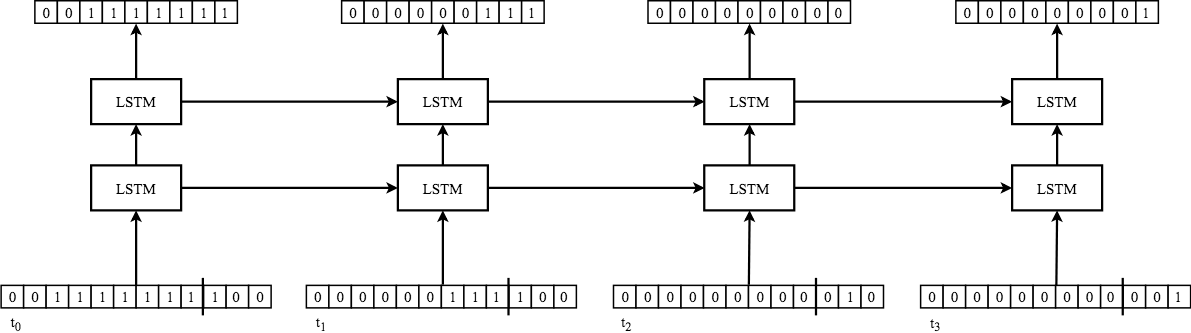
\includegraphics[max width=\textwidth]{sequential-model-temperature-symbols}
	\caption{A sequential model constrained to use symbols only. However, the symbols are encoded using temperature encoding. In this case the model is learning to perform 7 + 3. The output on the third time step (least significant time step) is all zeros to encode 0.}
	\label{fig:sequential-model-temperature-symbols}
\end{figure}

A similar dataset like the one used in Experiment 5 is used for this experiment. A subset of 80 combinations are selected for training from the 100 combinations of operands, making sure that each unique digit would be present at least once on either side of the addition operator. That same training set is also used for validation and as the test set of seen combinations. The remaining 20 combinations are used as the unseen combinations test set. Each model is trained and tested five times and the mean accuracy of each model is recorded when applying both the seen test set and the unseen test set on the trained model. Training is performed over 5000 epochs in batches of 10 using the Adam optimizer algorithm and the mean square error loss function with a learning rate of 0.001. 

\subsubsection{Results}

\begin{table}
	\center
	\caption{A comparison of the mean accuracy of each of the models trained using the temperature encoding when tested on the test set of \textbf{seen} combinations as well as the test set of \textbf{unseen} combinations.}
	\label{tab:experiment-7-results-table}
	\begin{tabular}{ |c|c|c| } 
		\hline
		Model & Accuracy - Seen (\%) & Accuracy - Unseen (\%)\\ 
		Model A & 100.0 & 90.0\\  
		Model B & 100.0 & 93.0\\  
		Model C & 100.0 & 86.0\\  
		\hline
	\end{tabular}
\end{table}

Table \ref{tab:experiment-7-results-table} shows the results obtained for each of the architectures trained. The table presents the mean accuracies of each architecture when tested on both the dataset of seen combinations and the dataset of unseen combinations. 

\subsubsection{Discussion}

\begin{figure}
	\centering
	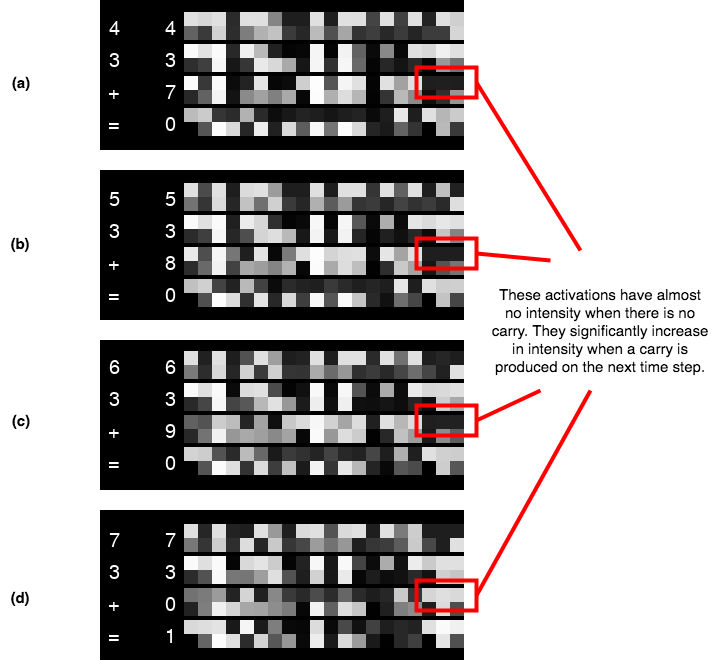
\includegraphics[max width=\textwidth]{activations-cluster-carry-temperature}
	\caption{A series of activations produced when applying examples from the unseen test set to Model A, trained using temperature encoded symbols. The activations show how the intensity in the top right region of the third time step indicates if a carry should be generated.}%
	\label{fig:activations-cluster-carry-temperature}%
\end{figure}

We can see from the results in Table \ref{tab:experiment-7-results-table} that the models perform perfectly on the training combinations and are also relatively successful at generalizing to the unseen combinations. This shows that the temperature encoded symbols that take into account the ordinal nature of the digits allow the recurrent neural networks to capture an algorithm that performs addition.

\begin{figure}%
	\centering
	\subfloat[Activations for 4 + 3]{{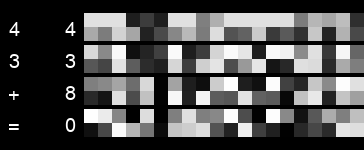
\includegraphics[width=0.5\textwidth]{activations-cluster-no-carry-4-3} }}%
	\subfloat[Activations for 5 + 3]{{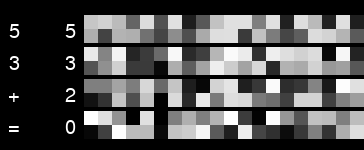
\includegraphics[width=0.5\textwidth]{activations-cluster-no-carry-5-3} }}%
	
	\subfloat[Activations for 6 + 3]{{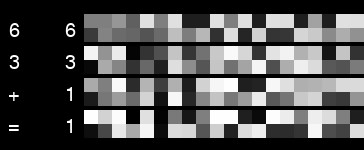
\includegraphics[width=0.5\textwidth]{activations-cluster-no-carry-6-3} }}%
	\subfloat[Activations for 7 + 3]{{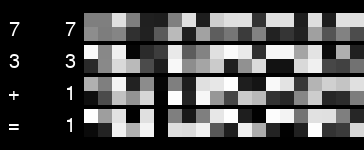
\includegraphics[width=0.5\textwidth]{activations-cluster-no-carry-7-3} }}%
	\caption{A series of activations produced when applying examples from the unseen test set to Model D of Experiment 5, trained using one-hot vector symbols. No discernible patterns are visible.}%
	\label{fig:activations-cluster-no-carry}%
\end{figure}

To further verify this conclusion, we generated activations clusters for a series of combinations from the unseen test set using Model A. Figure \ref{fig:activations-cluster-carry-temperature} shows the activations produced. In addition, Model D from the previous experiment (Experiment 5 in Section \ref{sec:experiment-5}) was retrained making sure that the same combinations shown in Figure \ref{fig:activations-cluster-carry-temperature} are part of the unseen test set. The activations for that model are shown in Figure \ref{fig:activations-cluster-no-carry}. The activations generated by the model trained using the temperature encoded symbols exhibit consistency among the same operands. Also, the region indicated at the top right end of the third time step shows a clearer carry forward signal than the one seen in Figure \ref{fig:activations-cluster-carry-temperature}. When we contrast these activations with the ones shown in Figure \ref{fig:activations-cluster-no-carry} we see that the model trained with one-hot vector symbols do not depict these clear patterns when applied to the unseen test set.

Experiments 5 and 6 show that symbols improve the accuracy of neural networks by aiding the learning algorithm in discovering a representation that capture some aspects of the algorithm that performs the operation. Temperature encoded symbols allow the models to capture more aspects. Specifically, the quantity and ordinal relationship of the operands. This results in better generalization. In the next and final experiment, we replicate Experiment 4 but this time, instead of using the one-hot vectors we use temperature encoded symbols.

\subsection{Experiment 7: Noisy Handwritten Digits with Temperature Encoded Symbols} \label{sec:experiment-7}

\subsubsection{Objective}

In Section \ref{sec:theory-approach-methodology-temperature-encoding} we explained our observation of how humans learn to perform arithmetic. We explained how children in particular learn to represent digits by mapping between the image of a digit and the image of familiar objects. These familiar objects (like apples for example) behave as symbols that convey both quantity and ordinal relationships. The human learner can then act on these symbols to produce a more accurate result. This process allows the human learner to generalize the solution to combinations of digits that they have not experienced before.

We believe a neural network model can be constructed that learns in a similar way. The network is provided a sequence of handwritten digits and an operator symbol. It is trained to develop an internal representation that can map between the image of the digit and a symbol that captures both the quantity and ordinal relationships represented by the digit (the temperature encoded symbol). The model is also trained to perform the arithmetic operation on the two digits. With deep recurrent neural networks, these two related tasks can be combined into one model that can learn to perform both with high accuracy.

The purpose of this experiment is to show that it is indeed possible to build such a model and that the use of symbols represented as temperature encodings can improve the accuracy of training on a restricted dataset as well as force the learning algorithm to discover a representation that can generalize to unseen combinations of digits. We also investigate how varying the amount of symbols present affects the accuracy of the model on the unseen test data.

\subsubsection{Method}

Five recurrent neural network models are developed for this experiment each having the same architecture. Figure \ref{fig:sequential-model-noisy-temperature} shows a diagram of the architecture used. The models accept a sequence of four 28x28 images. The first two images are of the MNIST handwritten digit operands, the third image is the operator (plus, minus, times and divide) consistently rendered in a standard font, and finally the fourth image is an equals sign. The model is trained so that when it sees the operands on each of the first two time steps, it outputs a temperature encoded symbol that represents the digit in the image. When the model is presented with the operator on the input, it performs the operation on the operands and then outputs a temperature encoded symbol that represents the least significant digit of the result. Finally, when the equals sign is presented, the model outputs a temperature encoded symbol representing the most significant digit of the result.

The neural network architecture used is composed of an input layer of 784 units for the 28x28 pixel images. Two hidden layers are used each consisting of 512 LSTM units. The output layer is a vector of nine elements to represent the temperature encoded results. The networks are trained using the Adam optimizer with the mean square error as the loss function and a learning rate of 0.001. Training is performed over 200 epochs in batches of 100 and the model performing best on the validation set is saved.

\begin{figure}
	\centering
	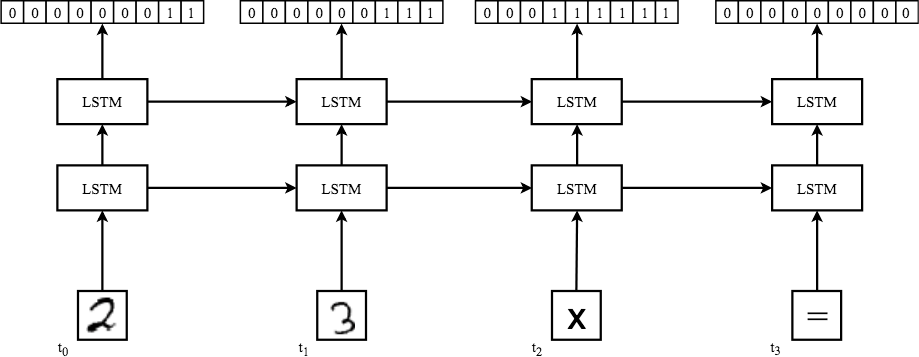
\includegraphics[max width=\textwidth]{sequential-model-noisy-temperature}
	\caption{A sequential model learning to perform arithmetic on images of handwritten digits in the presence of symbols. The symbols are provided on the outputs of the first two intermediate steps using temperature encoding. Here the model is performing multiplication on the combination: 2 x 3.}
	\label{fig:sequential-model-noisy-temperature}
\end{figure}

The same dataset used in Experiment 4 in Section \ref{sec:experiment-4} is also used for this experiment with the exception of replacing one-hot vector symbols with temperature encoded symbols. To recap, for each operator, the combinations of digits are split into a set of seen combinations that includes, 80\% of the combinations of digits. For each of the seen combinations, eight MNIST samples are selected. Four of these samples are used for training, two for validation and the remaining two for testing. The remaining 20\% of the combinations are reserved as the set of unseen combinations that are used to verify that the models have learned an algorithm of the operations. The dataset of seen combinations is replicated five times, each replica includes a different percentage of symbols present. The symbol spreads used are 0\%, 25\%, 50\%, 75\% and 100\%. The symbols were presented as output labels to the first two time steps. The model is trained to classify the handwritten digit with the aid of the symbol provided. When symbols are not provided, a vector composed of 0.5 dummy values is used instead. Each model is trained five times using 5-fold cross-validation.

\subsubsection{Results}

\begin{table}[p]
	\center
	\caption{A comparison of the mean accuracy and standard deviation along with the p-value of a hypothesis t-Test when compared to the 0\% symbols model when tested on the test set of \textbf{seen} combinations.}
	\label{tab:experiment-8-results-table-seen}
	\begin{tabular}{ |c|c|c|c| } 
		\hline
		\% Symbols Present & Accuracy (\%) & Standard Deviation  & p-value\\ 
		0\% & 41.55 & 0.0302 & NA \\  
		25\% & 51.30 & 0.0457 & 0.02311\\  
		50\% & 60.65 & 0.0379 & 0.00049 \\  
		75\% & 75.84 & 0.0587 & 0.00063\\  
		100\% & 84.26 & 0.0582 & 0.00018\\  
		\hline
	\end{tabular}
\end{table}

\begin{table}[p]
	\center
	\caption{A comparison of the mean accuracy and standard deviation along with the p-value of a hypothesis t-Test when compared to the 0\% symbols model when tested on the test set of \textbf{unseen} combinations.}
	\label{tab:experiment-8-results-table-unseen}
	\begin{tabular}{ |c|c|c|c| } 
		\hline
		\% Symbols Present & Accuracy (\%) & Standard Deviation  & p-value\\ 
		0\% & 4.62 & 0.0133 & NA \\  
		25\% & 25.53 & 0.0900 & 0.16889\\  
		50\% & 45.90 & 0.0319 & 0.00199 \\  
		75\% & 54.63 & 0.0324 & 0.0\\  
		100\% & 69.58 & 0.0694 & 0.00088\\  
		\hline
	\end{tabular}
\end{table}

\begin{figure}[p]
	\centering
	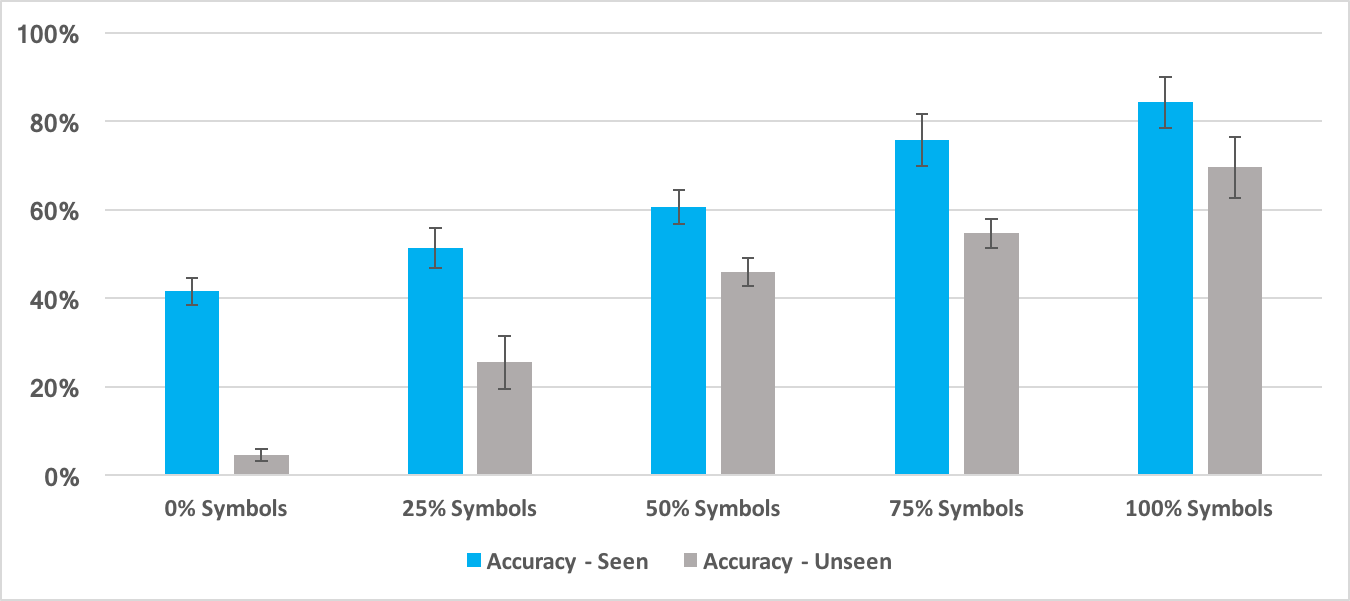
\includegraphics[max width=\textwidth]{experiment-8-results-chart-2}
	\caption{A comparison of the mean accuracy and 95\% confidence intervals for each of the models trained with 0\% to 100\% temperature encoded symbol presence when tested on both the test set of \textbf{seen} and \textbf{unseen} combinations.}
	\label{fig:experiment-8-results-chart}
\end{figure}

Table \ref{tab:experiment-8-results-table-seen} shows the results of testing the models on the test set of seen combinations. Similarly, Table \ref{tab:experiment-8-results-table-unseen} shows the results of testing the model on the test set of unseen combinations. The tables present the mean accuracy, standard deviation and the p-test score for each of the models developed. Figure \ref{fig:experiment-8-results-chart} depicts the mean accuracies along with the 95\% confidence intervals for all five models trained on both the seen and unseen test sets.

\subsubsection{Discussion}

The results show that increasing the number of symbols available per combination during training, improves the accuracy of the recurrent network when tested on combinations the model has seen during training. This result is comparable to Experiment 4 where we had a similar architecture and approach. However, we used a different representation for the symbols, namely temperature encoded vectors. More importantly the results show the accuracy on unseen combinations increases as more symbols are used during training. These results confirm the findings we've observed in several of our previous experiments and also supports our hypothesis that artificial neural networks similar to human learners can benefit from the presence of clear and concise symbols when training using limited datasets.

The results in this experiment show that the way the symbols are represented can have significant effect on the learning ability of the models. The one-hot vector representation was effective for learning a simple mapping function when all combinations of inputs were provided during training. However, it failed to capture the ordinal nature of the digits and therefore they were not able to discover a representation for an algorithm that can perform the arithmetic operations. By using temperature encoded symbols for the digits, the models are able to represent the arithmetic algorithm and generalize to unseen combinations of digits.

\section{Summary} \label{sec:theory-summary}

This chapter presented our basic hypothesis. The theory states that individual human learners struggle to learn new concepts through experimentation alone when the number of examples provided to them is limited. However, through interaction with other learners, common symbols for noisy concepts are shared that allows the learner to overcome the challenges in developing accurate models. We hypothesize that the introduction of such a symbolic channel to an artificial neural network model can also help the model achieve higher levels of accuracy when training with an impoverished dataset.

We also proposed a problem domain to validate this hypothesis, namely to teach artificial neural network models to perform arithmetic on images of handwritten digits. We first explained that the process of learning arithmetic operations can be modeled using sequential neural network architectures. We then presented two methods of supplying symbolic information to these models. Next, two theories were discussed on the role the symbols play in guiding the learning system towards discovering an optimum solution to the problem. Finally, we introduced a new form of symbolic representation, that of temperature encoding, that we believe will capture all aspects of learning to perform arithmetic and will therefore produce the best results. 
    \chapter{Conclusion} \label{sec:findings-and-conclusion}

In Chapter 1 we described the challenges that an individual human would have in learning to survive alone in the jungle. She or he would have to observe a large number of examples of a concept in order to learn the concept. We discussed how by using shared knowledge from other humans and relying on their past experiences, the lone learner is able to overcome learning from impoverished datasets. In traditional machine learning, computer systems do not have the benefit of shared knowledge and past experiences. They must rely on sufficient numbers of training examples to achieve the same level of accuracy as a human would.

In Chapter 3 we hypothesized that in the same manner that human learners are able to use shared knowledge to overcome the challenges they encounter while learning, machine learning systems can overcome impoverished datasets using shared knowledge. Our theory states that by introducing a clear and concise symbol channel, that is analogous to the knowledge shared by human learners, neural networks can overcome learning difficulties caused by small training sets and produce more accurate models. In Chapter 4, we presented a series of experiments that show how this theory can be applied to training recurrent neural networks to perform basic arithmetic on images of handwritten digits.

This final chapter starts by providing a summary of our findings and reflects on the objectives of our research (Section \ref{sec:findings-and-conclusion-summary-of-findings}). Next we describe the contributions made by our work (Section \ref{sec:findings-and-conclusion-research-contributions}). Finally, a list of suggested future work is presented in Section \ref{sec:findings-and-conclusion-future-work}.

\section{Summary of Findings} \label{sec:findings-and-conclusion-summary-of-findings}

Section \ref{sec:introduction-research-objective-scope-research-objective} stated two objectives for our research. The first objective was to validate the hypothesis by showing that neural networks trained using symbols perform significantly better than those trained without the presence of symbols. We started by developing several recurrent neural networks to perform arithmetic on images of noisy handwritten digits with the aid of symbols represented as one-hot vectors. Two methods of presenting the symbols to the networks were developed and tested. The first used a separate input channel alongside the noisy inputs. The other method trained the recurrent network to classify the incoming digits on the first time steps. The results obtained by these initial models confirmed our hypothesis, and therefore accomplished the first objective, by showing that regardless of the technique used to provide symbols, the models trained in the presence of symbols performed significantly better than those trained in the absence of symbols. We did not find much difference between the models trained with the explicit symbols and those trained by learning to classify the input.

The second objective was to explain the role of symbols. In Section \ref{sec:theory-approach}, we expanded the objective by stating that in order to explain why symbols improve the accuracy of trained models, we have to show that the presence of symbols allows the neural networks to discover a representation that captures an algorithm that performs arithmetic operations, just as with humans symbols allow learners to generalize to unseen concepts. Experiments 4 and 5 in Section \ref{sec:empirical-studies-explaining-the-role-of-symbols} showed that this is a difficult task for networks trained using one-hot vector symbols. We were however able to show that the networks trained with symbols were able to capture the carry forward process of addition. This led us to consider other representations for the symbols.

We theorized that a symbol must exhibit three characteristics in order to be able to guide a learner to a general solution. They must be able to represent quantity, ordinal relations and capture the operation being performed. By using temperature encoded symbols we were able to develop LSTM based recurrent neural networks that perform well on combinations of digits that were not seen during training. We therefore concluded that temperature encoded symbols are able to capture the three aspects needed by the symbols to discover an algorithm that can perform the arithmetic operation, thereby accomplishing the second objective. 

\section{Research Contributions} \label{sec:findings-and-conclusion-research-contributions}

This section lists contributions from our research that we believe to be novel and of significant interest.

\begin{itemize}
	\item Symbols that are presented on the network's output are as effective as those presented as an input to the neural network. Experiment 1 in Section \ref{sec:experiment-1} showed that the mean accuracy of the models trained with explicit symbols (NS), implicit symbols (NC) and both (NX) are statistically similar.
	\item The encoding used to represent symbols has a significant impact on the utility of the symbols and the overall effectiveness of the model. When we contrast the results obtained from Experiment 4 in Section \ref{sec:experiment-4} (one-hot vector symbols) with the ones obtained from Experiment 7 in Section \ref{sec:experiment-7} (temperature encoded symbols), not only do the models trained using temperature encoded symbols show significant improvement on the unseen test set, they also show slight improvement on the seen test set.
	\item Training neural networks with the aid of symbols takes more time than without the aid of symbols, contrary to our expectations. In Section \ref{sec:experiment-3}, we attributed this outcome to the possibility that it takes longer for the learning algorithm to find a suitable set of weights that fits both the symbolic data and the noisy handwritten digits.
\end{itemize}

\section{Future Work} \label{sec:findings-and-conclusion-future-work}

This final section suggests potential avenues for future development.

\begin{itemize}
	\item We focused our experimental efforts on training recurrent neural networks in the presence of symbols to learn arithmetic using images of handwritten digits. Future work can consider applying this theory of learning with symbols to other application domains. Specifically, natural language processing or medical imagery.
	\item Further qualitative investigations can be made similar to the ones presented in Experiment 5 in Section \ref{sec:experiment-5} and Experiment 6 in \ref{sec:experiment-6} to understand the development of algorithms in the neural network representation for operators other than addition.
	\item Our experiments used sequences of two operands. More experiments can be done to investigate the theory on longer sequences of operands. Specifically, experiments can be conducted to understand how the network would behave when the carry signal for addition would have to be carried over more than one place. Our current setup of using reverse Polish notation, although was not necessary for the experiments presented here, should eliminate the need for taking operator precedence into account.
	\item Instead of using recurrent neural networks and adding a symbolic channel, a feed forward neural network trained using a context sensitive multi-task learning (csMTL) approach like the one presented by Poirier and Silver\cite{silver2007context} could be investigated. The context input can be used to configure the network to either perform classification on the inputs or perform the operation. Our belief is the symbolic representation would be acquired implicitly by the network by learning to classify the operands within the one csMTL network.
\end{itemize}
    % APPENDICES
    % CHAPTER CONTENT END

    \bibliography{thesisbib}
\end{document}
